%% relatorio-mt-duas-fitas.tex
%% Trabalho: Operações lógicas sobre cadeias binárias
%% Máquina de Turing determinística de duas fitas (AND, OR, XOR)
%%
%% Compilar com:
%%   pdflatex relatorio-mt-duas-fitas.tex
%%   pdflatex relatorio-mt-duas-fitas.tex
%%
%% Arquivos na pasta do projeto:
%%   uftreport.cls, logos/            (classe e logo da UFT)
%%   mt_duas_fitas.py                 (código-fonte incluído no Capítulo 2)
%%   figuras/                         (diagramas/, execucao/ e resumo.png)

\documentclass[report, 12pt]{uftreport}

\usepackage{amsmath,amssymb}
\usepackage{longtable}
\usepackage{booktabs}
\usepackage{array}
\usepackage{float}
\usepackage{hyperref}

% Símbolos da máquina em fonte monoespaçada
\newcommand{\s}[1]{\texttt{#1}}
\hypersetup{colorlinks=true, urlcolor=blue, linkcolor=black}

% Folha de rosto sem o nome do autor (os autores aparecem só na capa)
\makeatletter
\renewcommand\makefrontpage{%
  \begin{center}
    \nohyphens{\bfseries\local@title}\par
  \end{center}
  \vfill
  \begin{flushright}
    \begin{minipage}{8.5cm}
      \setstretch{1}
      \frontpage@maintext
    \end{minipage}\par
  \end{flushright}
  \vfill
  \frontpage@bottomtext
}
\makeatother

% ── Metadados do documento ─────────────────────────────────────────────
\title{Operações Lógicas sobre Cadeias Binárias com Máquina de Turing de Duas Fitas}
\foreigntitle{Bitwise Logical Operations on Binary Strings with a Two-Tape Turing Machine}

\author{Matheus}{Silva Pontes}
\author{Lucas}{Monteiro de Carvalho}
% \author{Segundo}{Integrante}   % grupo de até 2 pessoas

\advisor{Prof.}{Alexandre}{Tadeu Rossini da Silva}{Dr.}

\department{CC}   % CC | LC | EC | EE

\class{Teoria da Computação -- 2026.2}

% \TRNumber{001}   % usado apenas com a opção techreport

\date{29}{9}{2026}   % dia, mês, ano



% ======================================================================
\begin{document}

% ── Elementos pré-textuais ─────────────────────────────────────────────
\frontmatter

\maketitle

\makefrontpage
\newpage

\tableofcontents

% ── Texto principal ────────────────────────────────────────────────────
\mainmatter

\ChapterStart{first}{Projeto da Máquina de Turing}

% ======================================================================
\chapter{Projeto da Máquina de Turing}
\label{cap:projeto}


\section{Definição formal}

Uma Máquina de Turing determinística de duas fitas pode ser definida
formalmente como uma extensão do modelo clássico de Máquina de Turing,
sendo representada por uma 7-tupla \cite{sipser}:

\[
M=(Q,\Sigma,\Gamma,\delta,q_0,B,F)
\]

onde:

\begin{itemize}
    \item $Q$ é um conjunto finito e não vazio de estados da máquina;
    \item $\Sigma$ é o alfabeto de entrada, formado pelos símbolos que podem
    aparecer inicialmente na fita de entrada;
    \item $\Gamma$ é o alfabeto da fita, contendo todos os símbolos que podem
    ser lidos ou escritos durante a execução da máquina, sendo
    $\Sigma \subseteq \Gamma$;
    \item $\delta$ é a função de transição da máquina;
    \item $q_0 \in Q$ é o estado inicial da computação;
    \item $B \in \Gamma$ é o símbolo branco, utilizado para representar
    posições vazias das fitas;
    \item $F \subseteq Q$ é o conjunto de estados finais ou estados de
    aceitação.
\end{itemize}

Por utilizar duas fitas, a máquina possui uma extensão da função de transição
tradicional, permitindo que a computação considere simultaneamente os símbolos
observados pelas cabeças das duas fitas. Máquinas de Turing com múltiplas fitas
possuem o mesmo poder computacional do modelo de uma única fita, porém permitem
uma descrição mais conveniente dos processos realizados
\cite{hopcroft}.

Dessa forma, a função de transição para uma Máquina de Turing determinística de
duas fitas é definida como:

\[
\delta: Q \times \Gamma \times \Gamma
\rightarrow
Q \times \Gamma \times \Gamma \times
\{L,R,S\} \times \{L,R,S\}
\]

onde:

\begin{itemize}
    \item $q \in Q$ representa o estado atual da máquina;
    \item $X_1,X_2 \in \Gamma$ representam os símbolos lidos pelas cabeças
    das fitas 1 e 2;
    \item $p \in Q$ representa o novo estado após a transição;
    \item $Y_1,Y_2 \in \Gamma$ representam os símbolos escritos nas fitas 1
    e 2;
    \item $D_1,D_2 \in \{L,R,S\}$ representam os movimentos das cabeças das
    fitas, sendo:
    \begin{itemize}
        \item $L$: movimento para a esquerda (\textit{Left});
        \item $R$: movimento para a direita (\textit{Right});
        \item $S$: permanece na mesma posição (\textit{Stay}).
    \end{itemize}
\end{itemize}

Assim, uma transição individual da máquina pode ser representada por:

\[
\delta(q,X_1,X_2)
=
(p,Y_1,Y_2,D_1,D_2)
\]

indicando que, estando no estado $q$ e lendo os símbolos $X_1$ e $X_2$ nas
duas fitas, a máquina muda para o estado $p$, escreve $Y_1$ e $Y_2$ nas
respectivas fitas e movimenta as cabeças conforme definido por $D_1$ e $D_2$.

Para a máquina desenvolvida neste trabalho, a fita 1 possui a função de
armazenar a entrada no formato:

\[
op\ w_1\#w_2
\]

onde $op \in \{A,O,X\}$ determina a operação lógica a ser executada. A fita 2
inicia completamente vazia e é utilizada exclusivamente para armazenar a
palavra resultante da operação bit a bit realizada entre $w_1$ e $w_2$.

Durante a computação, a máquina pode modificar temporariamente os símbolos da
fita 1 utilizando marcas auxiliares, porém a fita 2 não é utilizada como
memória auxiliar. Ao término da execução, a fita 2 contém somente o resultado
da operação lógica solicitada e a máquina encontra-se em um estado de
aceitação pertencente ao conjunto $F$.


\section{Alfabetos}

O alfabeto de entrada da máquina é definido por:

\[
\Sigma=\{0,1,A,O,X,\#\}
\]

onde os símbolos possuem as seguintes funções:

\begin{itemize}
    \item $0$ e $1$ representam os bits das palavras binárias;
    \item $A$, $O$ e $X$ representam as operações AND, OR e XOR;
    \item $\#$ representa o separador entre os operandos $w_1$ e $w_2$.
\end{itemize}


O alfabeto utilizado nas fitas é:

\[
\Gamma=\{0,1,A,O,X,\#,x,y,B\}
\]

Além dos símbolos presentes na entrada, a máquina utiliza símbolos auxiliares:

\begin{itemize}
    \item $B$: representa uma posição vazia da fita;
    \item $x$: marca temporariamente um bit originalmente igual a $0$ já
    processado;
    \item $y$: marca temporariamente um bit originalmente igual a $1$ já
    processado.
\end{itemize}

As marcações $x$ e $y$ permitem que a máquina controle quais bits já foram
utilizados durante a computação, mantendo a informação original para a etapa
de restauração da fita 1.


\section{Algoritmo em linguagem natural}

O funcionamento da Máquina de Turing ocorre através das seguintes etapas:

\begin{enumerate}

\item Inicialmente, a cabeça da fita 1 encontra-se posicionada sobre o
primeiro símbolo da entrada, enquanto a fita 2 permanece completamente vazia.

\item A máquina lê o primeiro símbolo da fita 1 para identificar a operação
a ser realizada:

\begin{itemize}
    \item símbolo $A$: direciona para o processamento AND;
    \item símbolo $O$: direciona para o processamento OR;
    \item símbolo $X$: direciona para o processamento XOR.
\end{itemize}

\item Após identificar a operação, a máquina procura o primeiro bit ainda não
processado da palavra $w_1$.

\item O bit encontrado é armazenado no estado atual da máquina, permitindo
que a informação seja mantida enquanto a cabeça percorre a fita até a segunda
palavra.

\item A máquina desloca-se pela fita 1 até encontrar o símbolo $\#$ e inicia
a busca pelo bit correspondente da palavra $w_2$.

\item Ao encontrar o próximo bit não processado de $w_2$, a máquina realiza a
operação lógica correspondente e escreve o resultado na fita 2.

\item Os bits utilizados são marcados com os símbolos auxiliares $x$ e $y$,
impedindo que sejam utilizados novamente.

\item A cabeça retorna para a região inicial da fita 1 e o processo é repetido
até que todos os bits das duas palavras tenham sido processados.

\item Após finalizar a computação, a máquina restaura as marcações temporárias
da fita 1, substituindo:

\[
x \rightarrow 0
\]

\[
y \rightarrow 1
\]

\item Finalmente, a máquina alcança o estado de aceitação, deixando a fita 2
contendo exclusivamente o resultado da operação lógica.

\end{enumerate}


\section{Identificação da operação}

A identificação da operação lógica é realizada pela própria Máquina de
Turing através da leitura do primeiro símbolo presente na fita 1.

No estado inicial $q_0$, a máquina verifica o símbolo encontrado e direciona a
execução para o conjunto de estados correspondente:

\[
\delta(q_0,A,B)=(q_{and},A,B,R,S)
\]

Quando o símbolo lido é $A$, a máquina entra no bloco responsável pela
operação AND.

\[
\delta(q_0,O,B)=(q_{or},O,B,R,S)
\]

Quando o símbolo lido é $O$, a execução é direcionada para o bloco da
operação OR.

\[
\delta(q_0,X,B)=(q_{xor},X,B,R,S)
\]

Quando o símbolo lido é $X$, a máquina utiliza o bloco responsável pela
operação XOR.

O modelo de Máquina de Turing foi originalmente proposto por Alan Turing como
uma formalização matemática do conceito de computabilidade
\cite{turing}. A partir desse modelo, diferentes extensões, como máquinas de
múltiplas fitas, foram desenvolvidas mantendo os mesmos fundamentos teóricos
\cite{sipser}.

Dessa forma, a operação não é informada externamente pelo programa. A própria
máquina determina seu comportamento através da leitura da entrada, mantendo
o modelo formal de uma Máquina de Turing determinística de duas fitas.
\section{Localização e processamento dos bits}

Os dois operandos são percorridos em ``zigue-zague''. A cada rodada:
\begin{itemize}
  \item o bit de $w_1$ a ser usado é o \textbf{primeiro não marcado} depois do
        símbolo da operação;
  \item o bit de $w_2$ a ser usado é o \textbf{primeiro não marcado} depois do
        \s{\#}.
\end{itemize}

Como cada rodada marca exatamente um bit de $w_1$ e um bit de $w_2$, na rodada $i$ a
máquina combina o $i$-ésimo bit de $w_1$ com o $i$-ésimo bit de $w_2$ e escreve o
$i$-ésimo bit do resultado na posição $i-1$ da fita 2. O valor do bit de $w_1$ viaja
no estado (\s{q\_op\_0} ou \s{q\_op\_1}) e a operação viaja no prefixo do estado
(\s{and}, \s{or}, \s{xor}). A Tabela~\ref{tab:rodadas} ilustra o processo.

\begin{table}[H]
\centering
\caption{Rodadas de processamento para a entrada \s{A101\#110}}
\label{tab:rodadas}
\begin{tabular}{llll}
\toprule
\textbf{Rodada} & \textbf{Fita 1 (início)} & \textbf{Par processado} & \textbf{Fita 2 (após)} \\
\midrule
1 & \s{A101\#110} & $1 \land 1 = 1$ & \s{1} \\
2 & \s{Ay01\#y10} & $0 \land 1 = 0$ & \s{10} \\
3 & \s{Ayx1\#yy0} & $1 \land 0 = 0$ & \s{100} \\
fim & \s{Ayxy\#yyx} & restaura $\to$ \s{A101\#110} & \s{100} \\
\bottomrule
\end{tabular}
\end{table}

\subsection{Entradas inválidas}

Se $|w_1| > |w_2|$, algum estado \s{q\_op\_bw2} encontra $B$ sem transição e a
máquina rejeita. Se $|w_1| < |w_2|$, \s{q\_rest\_dir} encontra um bit \s{0}/\s{1}
não marcado em $w_2$, também sem transição, e a máquina rejeita. Símbolos fora de
$\Sigma$ ou ausência de \s{\#} levam ao mesmo resultado.

\subsection{Custo}

Para $|w_1| = |w_2| = n$, cada rodada percorre no máximo toda a entrada duas vezes;
portanto, a máquina executa $O(n^2)$ passos (por exemplo, 41 passos para $n=3$ e 85
para $n=5$).

\section{Estados e finalidade}
\label{sec:estados}

Na Tabela~\ref{tab:estados}, \s{op} $\in \{\s{and}, \s{or}, \s{xor}\}$ e
$b \in \{0,1\}$. Cada linha com \s{op} representa três estados (um por operação) e
cada linha com $b$ representa dois.

\begin{longtable}{>{\raggedright\arraybackslash}p{3.0cm} c >{\raggedright\arraybackslash}p{8.6cm}}
\caption{Estados da máquina e sua finalidade}\label{tab:estados}\\
\toprule
\textbf{Estado} & \textbf{Qtd.} & \textbf{Finalidade} \\
\midrule
\endfirsthead
\toprule
\textbf{Estado} & \textbf{Qtd.} & \textbf{Finalidade} \\
\midrule
\endhead
\s{q0} & 1 & Estado inicial. Lê o símbolo da operação e desvia para o bloco correspondente. \\
\s{q\_op} & 3 & Cabeça 1 sobre o próximo bit não processado de $w_1$. Marca o bit e guarda seu valor no estado; se ler \s{\#}, todos os bits foram processados e começa a restauração. \\
\s{q\_op\_b} & 6 & Guarda que o bit atual de $w_1$ vale $b$. Anda para a direita sobre $w_1$ até o \s{\#}. \\
\s{q\_op\_bw2} & 6 & Ainda guardando $b$, pula os bits já marcados de $w_2$. No primeiro bit não marcado $c$: marca-o, escreve $b \mathbin{op} c$ na fita 2 e avança a cabeça 2. \\
\s{q\_op\_volta2} & 3 & Volta para a esquerda sobre os bits marcados de $w_2$ até o \s{\#}. \\
\s{q\_op\_volta1} & 3 & Volta para a esquerda sobre os bits não marcados de $w_1$ até achar um bit marcado ou o símbolo da operação; dá um passo à direita e retorna a \s{q\_op}. \\
\s{q\_rest\_dir} & 1 & Percorre $w_2$ para a direita desfazendo as marcas (\s{x}$\to$\s{0}, \s{y}$\to$\s{1}) até o branco. \\
\s{q\_rest\_esq} & 1 & Volta para a esquerda desfazendo as marcas de $w_1$ até o símbolo da operação. \\
\s{q\_aceita} & 1 & Estado final (de aceitação). Não há transições saindo dele. \\
\midrule
\textbf{Total} & \textbf{25} & \\
\bottomrule
\end{longtable}

\section{Tabela completa da função de transição}
\label{sec:delta}

A Tabela~\ref{tab:delta} lista as 89 transições. Ela foi gerada a partir do mesmo
dicionário \s{transicoes} usado no programa Python do
Capítulo~\ref{cap:implementacao}, garantindo que a máquina do projeto é exatamente a
máquina executada.

{\small
\begin{longtable}{r l l}
\caption{Função de transição $\delta$ completa}\label{tab:delta}\\
\toprule
\textbf{\#} & $\boldsymbol{\delta(q, X_1, X_2)}$ & $\boldsymbol{(p, Y_1, Y_2, D_1, D_2)}$ \\
\midrule
\endfirsthead
\toprule
\textbf{\#} & $\boldsymbol{\delta(q, X_1, X_2)}$ & $\boldsymbol{(p, Y_1, Y_2, D_1, D_2)}$ \\
\midrule
\endhead
\midrule
\multicolumn{3}{r}{\footnotesize continua na próxima página}\\
\endfoot
\bottomrule
\endlastfoot
1 & $\delta$(\texttt{q0}, \texttt{A}, \texttt{B}) & (\texttt{q\_and}, \texttt{A}, \texttt{B}, \texttt{R}, \texttt{S}) \\
2 & $\delta$(\texttt{q0}, \texttt{O}, \texttt{B}) & (\texttt{q\_or}, \texttt{O}, \texttt{B}, \texttt{R}, \texttt{S}) \\
3 & $\delta$(\texttt{q0}, \texttt{X}, \texttt{B}) & (\texttt{q\_xor}, \texttt{X}, \texttt{B}, \texttt{R}, \texttt{S}) \\
\midrule
4 & $\delta$(\texttt{q\_and}, \texttt{0}, \texttt{B}) & (\texttt{q\_and\_0}, \texttt{x}, \texttt{B}, \texttt{R}, \texttt{S}) \\
5 & $\delta$(\texttt{q\_and}, \texttt{1}, \texttt{B}) & (\texttt{q\_and\_1}, \texttt{y}, \texttt{B}, \texttt{R}, \texttt{S}) \\
6 & $\delta$(\texttt{q\_and}, \texttt{\#}, \texttt{B}) & (\texttt{q\_rest\_dir}, \texttt{\#}, \texttt{B}, \texttt{R}, \texttt{S}) \\
\midrule
7 & $\delta$(\texttt{q\_and\_0}, \texttt{0}, \texttt{B}) & (\texttt{q\_and\_0}, \texttt{0}, \texttt{B}, \texttt{R}, \texttt{S}) \\
8 & $\delta$(\texttt{q\_and\_0}, \texttt{1}, \texttt{B}) & (\texttt{q\_and\_0}, \texttt{1}, \texttt{B}, \texttt{R}, \texttt{S}) \\
9 & $\delta$(\texttt{q\_and\_0}, \texttt{\#}, \texttt{B}) & (\texttt{q\_and\_0w2}, \texttt{\#}, \texttt{B}, \texttt{R}, \texttt{S}) \\
\midrule
10 & $\delta$(\texttt{q\_and\_0w2}, \texttt{x}, \texttt{B}) & (\texttt{q\_and\_0w2}, \texttt{x}, \texttt{B}, \texttt{R}, \texttt{S}) \\
11 & $\delta$(\texttt{q\_and\_0w2}, \texttt{y}, \texttt{B}) & (\texttt{q\_and\_0w2}, \texttt{y}, \texttt{B}, \texttt{R}, \texttt{S}) \\
12 & $\delta$(\texttt{q\_and\_0w2}, \texttt{0}, \texttt{B}) & (\texttt{q\_and\_volta2}, \texttt{x}, \texttt{0}, \texttt{L}, \texttt{R}) \\
13 & $\delta$(\texttt{q\_and\_0w2}, \texttt{1}, \texttt{B}) & (\texttt{q\_and\_volta2}, \texttt{y}, \texttt{0}, \texttt{L}, \texttt{R}) \\
\midrule
14 & $\delta$(\texttt{q\_and\_1}, \texttt{0}, \texttt{B}) & (\texttt{q\_and\_1}, \texttt{0}, \texttt{B}, \texttt{R}, \texttt{S}) \\
15 & $\delta$(\texttt{q\_and\_1}, \texttt{1}, \texttt{B}) & (\texttt{q\_and\_1}, \texttt{1}, \texttt{B}, \texttt{R}, \texttt{S}) \\
16 & $\delta$(\texttt{q\_and\_1}, \texttt{\#}, \texttt{B}) & (\texttt{q\_and\_1w2}, \texttt{\#}, \texttt{B}, \texttt{R}, \texttt{S}) \\
\midrule
17 & $\delta$(\texttt{q\_and\_1w2}, \texttt{x}, \texttt{B}) & (\texttt{q\_and\_1w2}, \texttt{x}, \texttt{B}, \texttt{R}, \texttt{S}) \\
18 & $\delta$(\texttt{q\_and\_1w2}, \texttt{y}, \texttt{B}) & (\texttt{q\_and\_1w2}, \texttt{y}, \texttt{B}, \texttt{R}, \texttt{S}) \\
19 & $\delta$(\texttt{q\_and\_1w2}, \texttt{0}, \texttt{B}) & (\texttt{q\_and\_volta2}, \texttt{x}, \texttt{0}, \texttt{L}, \texttt{R}) \\
20 & $\delta$(\texttt{q\_and\_1w2}, \texttt{1}, \texttt{B}) & (\texttt{q\_and\_volta2}, \texttt{y}, \texttt{1}, \texttt{L}, \texttt{R}) \\
\midrule
21 & $\delta$(\texttt{q\_and\_volta2}, \texttt{x}, \texttt{B}) & (\texttt{q\_and\_volta2}, \texttt{x}, \texttt{B}, \texttt{L}, \texttt{S}) \\
22 & $\delta$(\texttt{q\_and\_volta2}, \texttt{y}, \texttt{B}) & (\texttt{q\_and\_volta2}, \texttt{y}, \texttt{B}, \texttt{L}, \texttt{S}) \\
23 & $\delta$(\texttt{q\_and\_volta2}, \texttt{\#}, \texttt{B}) & (\texttt{q\_and\_volta1}, \texttt{\#}, \texttt{B}, \texttt{L}, \texttt{S}) \\
\midrule
24 & $\delta$(\texttt{q\_and\_volta1}, \texttt{0}, \texttt{B}) & (\texttt{q\_and\_volta1}, \texttt{0}, \texttt{B}, \texttt{L}, \texttt{S}) \\
25 & $\delta$(\texttt{q\_and\_volta1}, \texttt{1}, \texttt{B}) & (\texttt{q\_and\_volta1}, \texttt{1}, \texttt{B}, \texttt{L}, \texttt{S}) \\
26 & $\delta$(\texttt{q\_and\_volta1}, \texttt{x}, \texttt{B}) & (\texttt{q\_and}, \texttt{x}, \texttt{B}, \texttt{R}, \texttt{S}) \\
27 & $\delta$(\texttt{q\_and\_volta1}, \texttt{y}, \texttt{B}) & (\texttt{q\_and}, \texttt{y}, \texttt{B}, \texttt{R}, \texttt{S}) \\
28 & $\delta$(\texttt{q\_and\_volta1}, \texttt{A}, \texttt{B}) & (\texttt{q\_and}, \texttt{A}, \texttt{B}, \texttt{R}, \texttt{S}) \\
\midrule
29 & $\delta$(\texttt{q\_or}, \texttt{0}, \texttt{B}) & (\texttt{q\_or\_0}, \texttt{x}, \texttt{B}, \texttt{R}, \texttt{S}) \\
30 & $\delta$(\texttt{q\_or}, \texttt{1}, \texttt{B}) & (\texttt{q\_or\_1}, \texttt{y}, \texttt{B}, \texttt{R}, \texttt{S}) \\
31 & $\delta$(\texttt{q\_or}, \texttt{\#}, \texttt{B}) & (\texttt{q\_rest\_dir}, \texttt{\#}, \texttt{B}, \texttt{R}, \texttt{S}) \\
\midrule
32 & $\delta$(\texttt{q\_or\_0}, \texttt{0}, \texttt{B}) & (\texttt{q\_or\_0}, \texttt{0}, \texttt{B}, \texttt{R}, \texttt{S}) \\
33 & $\delta$(\texttt{q\_or\_0}, \texttt{1}, \texttt{B}) & (\texttt{q\_or\_0}, \texttt{1}, \texttt{B}, \texttt{R}, \texttt{S}) \\
34 & $\delta$(\texttt{q\_or\_0}, \texttt{\#}, \texttt{B}) & (\texttt{q\_or\_0w2}, \texttt{\#}, \texttt{B}, \texttt{R}, \texttt{S}) \\
\midrule
35 & $\delta$(\texttt{q\_or\_0w2}, \texttt{x}, \texttt{B}) & (\texttt{q\_or\_0w2}, \texttt{x}, \texttt{B}, \texttt{R}, \texttt{S}) \\
36 & $\delta$(\texttt{q\_or\_0w2}, \texttt{y}, \texttt{B}) & (\texttt{q\_or\_0w2}, \texttt{y}, \texttt{B}, \texttt{R}, \texttt{S}) \\
37 & $\delta$(\texttt{q\_or\_0w2}, \texttt{0}, \texttt{B}) & (\texttt{q\_or\_volta2}, \texttt{x}, \texttt{0}, \texttt{L}, \texttt{R}) \\
38 & $\delta$(\texttt{q\_or\_0w2}, \texttt{1}, \texttt{B}) & (\texttt{q\_or\_volta2}, \texttt{y}, \texttt{1}, \texttt{L}, \texttt{R}) \\
\midrule
39 & $\delta$(\texttt{q\_or\_1}, \texttt{0}, \texttt{B}) & (\texttt{q\_or\_1}, \texttt{0}, \texttt{B}, \texttt{R}, \texttt{S}) \\
40 & $\delta$(\texttt{q\_or\_1}, \texttt{1}, \texttt{B}) & (\texttt{q\_or\_1}, \texttt{1}, \texttt{B}, \texttt{R}, \texttt{S}) \\
41 & $\delta$(\texttt{q\_or\_1}, \texttt{\#}, \texttt{B}) & (\texttt{q\_or\_1w2}, \texttt{\#}, \texttt{B}, \texttt{R}, \texttt{S}) \\
\midrule
42 & $\delta$(\texttt{q\_or\_1w2}, \texttt{x}, \texttt{B}) & (\texttt{q\_or\_1w2}, \texttt{x}, \texttt{B}, \texttt{R}, \texttt{S}) \\
43 & $\delta$(\texttt{q\_or\_1w2}, \texttt{y}, \texttt{B}) & (\texttt{q\_or\_1w2}, \texttt{y}, \texttt{B}, \texttt{R}, \texttt{S}) \\
44 & $\delta$(\texttt{q\_or\_1w2}, \texttt{0}, \texttt{B}) & (\texttt{q\_or\_volta2}, \texttt{x}, \texttt{1}, \texttt{L}, \texttt{R}) \\
45 & $\delta$(\texttt{q\_or\_1w2}, \texttt{1}, \texttt{B}) & (\texttt{q\_or\_volta2}, \texttt{y}, \texttt{1}, \texttt{L}, \texttt{R}) \\
\midrule
46 & $\delta$(\texttt{q\_or\_volta2}, \texttt{x}, \texttt{B}) & (\texttt{q\_or\_volta2}, \texttt{x}, \texttt{B}, \texttt{L}, \texttt{S}) \\
47 & $\delta$(\texttt{q\_or\_volta2}, \texttt{y}, \texttt{B}) & (\texttt{q\_or\_volta2}, \texttt{y}, \texttt{B}, \texttt{L}, \texttt{S}) \\
48 & $\delta$(\texttt{q\_or\_volta2}, \texttt{\#}, \texttt{B}) & (\texttt{q\_or\_volta1}, \texttt{\#}, \texttt{B}, \texttt{L}, \texttt{S}) \\
\midrule
49 & $\delta$(\texttt{q\_or\_volta1}, \texttt{0}, \texttt{B}) & (\texttt{q\_or\_volta1}, \texttt{0}, \texttt{B}, \texttt{L}, \texttt{S}) \\
50 & $\delta$(\texttt{q\_or\_volta1}, \texttt{1}, \texttt{B}) & (\texttt{q\_or\_volta1}, \texttt{1}, \texttt{B}, \texttt{L}, \texttt{S}) \\
51 & $\delta$(\texttt{q\_or\_volta1}, \texttt{x}, \texttt{B}) & (\texttt{q\_or}, \texttt{x}, \texttt{B}, \texttt{R}, \texttt{S}) \\
52 & $\delta$(\texttt{q\_or\_volta1}, \texttt{y}, \texttt{B}) & (\texttt{q\_or}, \texttt{y}, \texttt{B}, \texttt{R}, \texttt{S}) \\
53 & $\delta$(\texttt{q\_or\_volta1}, \texttt{O}, \texttt{B}) & (\texttt{q\_or}, \texttt{O}, \texttt{B}, \texttt{R}, \texttt{S}) \\
\midrule
54 & $\delta$(\texttt{q\_xor}, \texttt{0}, \texttt{B}) & (\texttt{q\_xor\_0}, \texttt{x}, \texttt{B}, \texttt{R}, \texttt{S}) \\
55 & $\delta$(\texttt{q\_xor}, \texttt{1}, \texttt{B}) & (\texttt{q\_xor\_1}, \texttt{y}, \texttt{B}, \texttt{R}, \texttt{S}) \\
56 & $\delta$(\texttt{q\_xor}, \texttt{\#}, \texttt{B}) & (\texttt{q\_rest\_dir}, \texttt{\#}, \texttt{B}, \texttt{R}, \texttt{S}) \\
\midrule
57 & $\delta$(\texttt{q\_xor\_0}, \texttt{0}, \texttt{B}) & (\texttt{q\_xor\_0}, \texttt{0}, \texttt{B}, \texttt{R}, \texttt{S}) \\
58 & $\delta$(\texttt{q\_xor\_0}, \texttt{1}, \texttt{B}) & (\texttt{q\_xor\_0}, \texttt{1}, \texttt{B}, \texttt{R}, \texttt{S}) \\
59 & $\delta$(\texttt{q\_xor\_0}, \texttt{\#}, \texttt{B}) & (\texttt{q\_xor\_0w2}, \texttt{\#}, \texttt{B}, \texttt{R}, \texttt{S}) \\
\midrule
60 & $\delta$(\texttt{q\_xor\_0w2}, \texttt{x}, \texttt{B}) & (\texttt{q\_xor\_0w2}, \texttt{x}, \texttt{B}, \texttt{R}, \texttt{S}) \\
61 & $\delta$(\texttt{q\_xor\_0w2}, \texttt{y}, \texttt{B}) & (\texttt{q\_xor\_0w2}, \texttt{y}, \texttt{B}, \texttt{R}, \texttt{S}) \\
62 & $\delta$(\texttt{q\_xor\_0w2}, \texttt{0}, \texttt{B}) & (\texttt{q\_xor\_volta2}, \texttt{x}, \texttt{0}, \texttt{L}, \texttt{R}) \\
63 & $\delta$(\texttt{q\_xor\_0w2}, \texttt{1}, \texttt{B}) & (\texttt{q\_xor\_volta2}, \texttt{y}, \texttt{1}, \texttt{L}, \texttt{R}) \\
\midrule
64 & $\delta$(\texttt{q\_xor\_1}, \texttt{0}, \texttt{B}) & (\texttt{q\_xor\_1}, \texttt{0}, \texttt{B}, \texttt{R}, \texttt{S}) \\
65 & $\delta$(\texttt{q\_xor\_1}, \texttt{1}, \texttt{B}) & (\texttt{q\_xor\_1}, \texttt{1}, \texttt{B}, \texttt{R}, \texttt{S}) \\
66 & $\delta$(\texttt{q\_xor\_1}, \texttt{\#}, \texttt{B}) & (\texttt{q\_xor\_1w2}, \texttt{\#}, \texttt{B}, \texttt{R}, \texttt{S}) \\
\midrule
67 & $\delta$(\texttt{q\_xor\_1w2}, \texttt{x}, \texttt{B}) & (\texttt{q\_xor\_1w2}, \texttt{x}, \texttt{B}, \texttt{R}, \texttt{S}) \\
68 & $\delta$(\texttt{q\_xor\_1w2}, \texttt{y}, \texttt{B}) & (\texttt{q\_xor\_1w2}, \texttt{y}, \texttt{B}, \texttt{R}, \texttt{S}) \\
69 & $\delta$(\texttt{q\_xor\_1w2}, \texttt{0}, \texttt{B}) & (\texttt{q\_xor\_volta2}, \texttt{x}, \texttt{1}, \texttt{L}, \texttt{R}) \\
70 & $\delta$(\texttt{q\_xor\_1w2}, \texttt{1}, \texttt{B}) & (\texttt{q\_xor\_volta2}, \texttt{y}, \texttt{0}, \texttt{L}, \texttt{R}) \\
\midrule
71 & $\delta$(\texttt{q\_xor\_volta2}, \texttt{x}, \texttt{B}) & (\texttt{q\_xor\_volta2}, \texttt{x}, \texttt{B}, \texttt{L}, \texttt{S}) \\
72 & $\delta$(\texttt{q\_xor\_volta2}, \texttt{y}, \texttt{B}) & (\texttt{q\_xor\_volta2}, \texttt{y}, \texttt{B}, \texttt{L}, \texttt{S}) \\
73 & $\delta$(\texttt{q\_xor\_volta2}, \texttt{\#}, \texttt{B}) & (\texttt{q\_xor\_volta1}, \texttt{\#}, \texttt{B}, \texttt{L}, \texttt{S}) \\
\midrule
74 & $\delta$(\texttt{q\_xor\_volta1}, \texttt{0}, \texttt{B}) & (\texttt{q\_xor\_volta1}, \texttt{0}, \texttt{B}, \texttt{L}, \texttt{S}) \\
75 & $\delta$(\texttt{q\_xor\_volta1}, \texttt{1}, \texttt{B}) & (\texttt{q\_xor\_volta1}, \texttt{1}, \texttt{B}, \texttt{L}, \texttt{S}) \\
76 & $\delta$(\texttt{q\_xor\_volta1}, \texttt{x}, \texttt{B}) & (\texttt{q\_xor}, \texttt{x}, \texttt{B}, \texttt{R}, \texttt{S}) \\
77 & $\delta$(\texttt{q\_xor\_volta1}, \texttt{y}, \texttt{B}) & (\texttt{q\_xor}, \texttt{y}, \texttt{B}, \texttt{R}, \texttt{S}) \\
78 & $\delta$(\texttt{q\_xor\_volta1}, \texttt{X}, \texttt{B}) & (\texttt{q\_xor}, \texttt{X}, \texttt{B}, \texttt{R}, \texttt{S}) \\
\midrule
79 & $\delta$(\texttt{q\_rest\_dir}, \texttt{x}, \texttt{B}) & (\texttt{q\_rest\_dir}, \texttt{0}, \texttt{B}, \texttt{R}, \texttt{S}) \\
80 & $\delta$(\texttt{q\_rest\_dir}, \texttt{y}, \texttt{B}) & (\texttt{q\_rest\_dir}, \texttt{1}, \texttt{B}, \texttt{R}, \texttt{S}) \\
81 & $\delta$(\texttt{q\_rest\_dir}, \texttt{B}, \texttt{B}) & (\texttt{q\_rest\_esq}, \texttt{B}, \texttt{B}, \texttt{L}, \texttt{S}) \\
\midrule
82 & $\delta$(\texttt{q\_rest\_esq}, \texttt{x}, \texttt{B}) & (\texttt{q\_rest\_esq}, \texttt{0}, \texttt{B}, \texttt{L}, \texttt{S}) \\
83 & $\delta$(\texttt{q\_rest\_esq}, \texttt{y}, \texttt{B}) & (\texttt{q\_rest\_esq}, \texttt{1}, \texttt{B}, \texttt{L}, \texttt{S}) \\
84 & $\delta$(\texttt{q\_rest\_esq}, \texttt{0}, \texttt{B}) & (\texttt{q\_rest\_esq}, \texttt{0}, \texttt{B}, \texttt{L}, \texttt{S}) \\
85 & $\delta$(\texttt{q\_rest\_esq}, \texttt{1}, \texttt{B}) & (\texttt{q\_rest\_esq}, \texttt{1}, \texttt{B}, \texttt{L}, \texttt{S}) \\
86 & $\delta$(\texttt{q\_rest\_esq}, \texttt{\#}, \texttt{B}) & (\texttt{q\_rest\_esq}, \texttt{\#}, \texttt{B}, \texttt{L}, \texttt{S}) \\
87 & $\delta$(\texttt{q\_rest\_esq}, \texttt{A}, \texttt{B}) & (\texttt{q\_aceita}, \texttt{A}, \texttt{B}, \texttt{S}, \texttt{S}) \\
88 & $\delta$(\texttt{q\_rest\_esq}, \texttt{O}, \texttt{B}) & (\texttt{q\_aceita}, \texttt{O}, \texttt{B}, \texttt{S}, \texttt{S}) \\
89 & $\delta$(\texttt{q\_rest\_esq}, \texttt{X}, \texttt{B}) & (\texttt{q\_aceita}, \texttt{X}, \texttt{B}, \texttt{S}, \texttt{S}) \\
\end{longtable}
}

\clearpage
\section{Diagrama de transição}

Nas Figuras~\ref{fig:diagrama} e~\ref{fig:blocos}, cada aresta é rotulada por
``$X_1, X_2 \to Y_1, Y_2, D_1, D_2$''. Arestas com vários rótulos agrupam transições
com o mesmo estado de origem e destino. O estado de aceitação está em círculo duplo.

\begin{figure}[H]
\centering
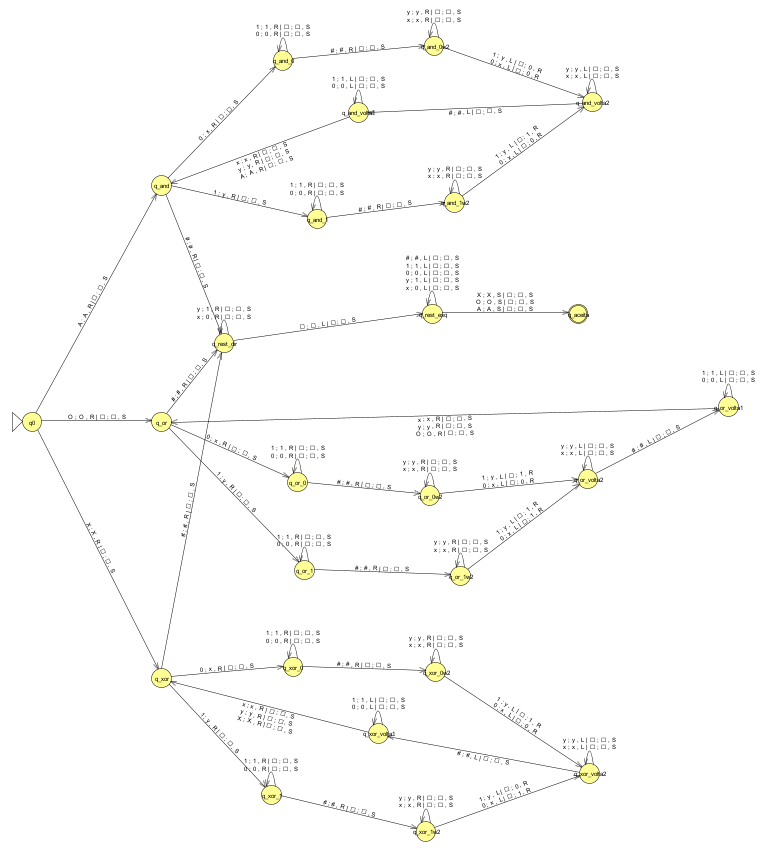
\includegraphics[width=\linewidth,height=0.72\textheight,keepaspectratio]{figuras/diagramas/diag_completo.png}
\caption{Diagrama completo da máquina (25 estados, 89 transições)}
\label{fig:diagrama}
\end{figure}

\begin{figure}[H]
\centering
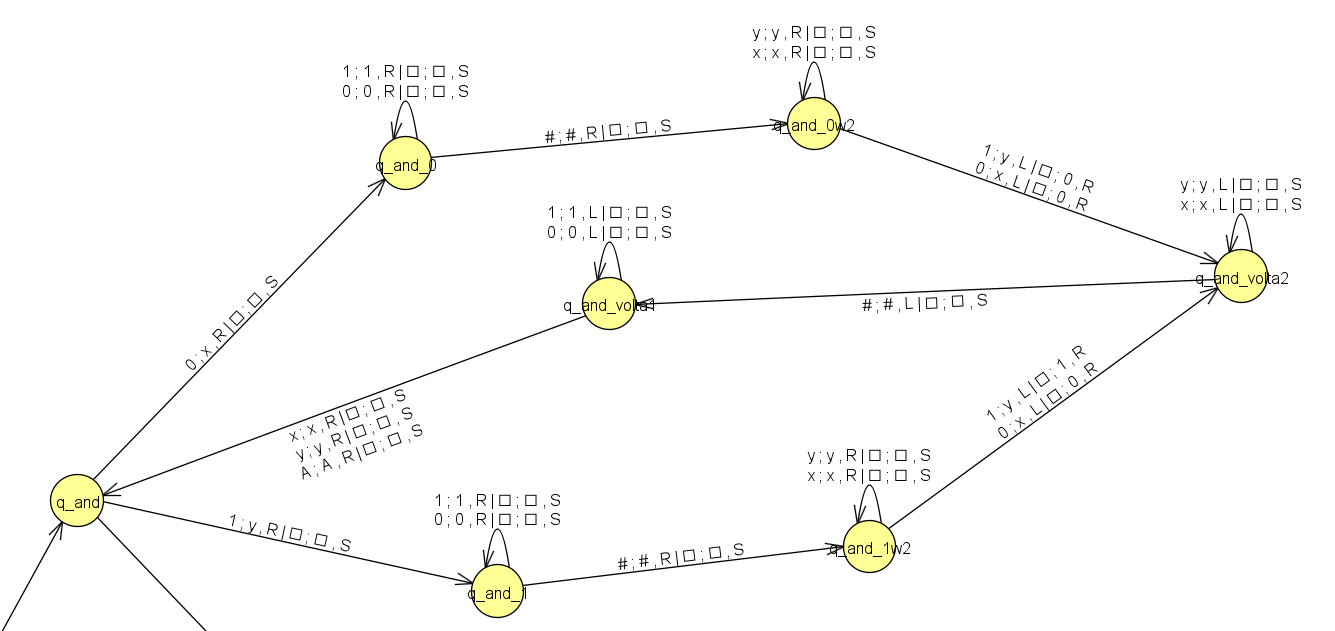
\includegraphics[width=\linewidth,height=0.22\textheight,keepaspectratio]{figuras/diagramas/diag_and.png}\\[0.2em]
{\small (a) Bloco AND}\\[0.8em]
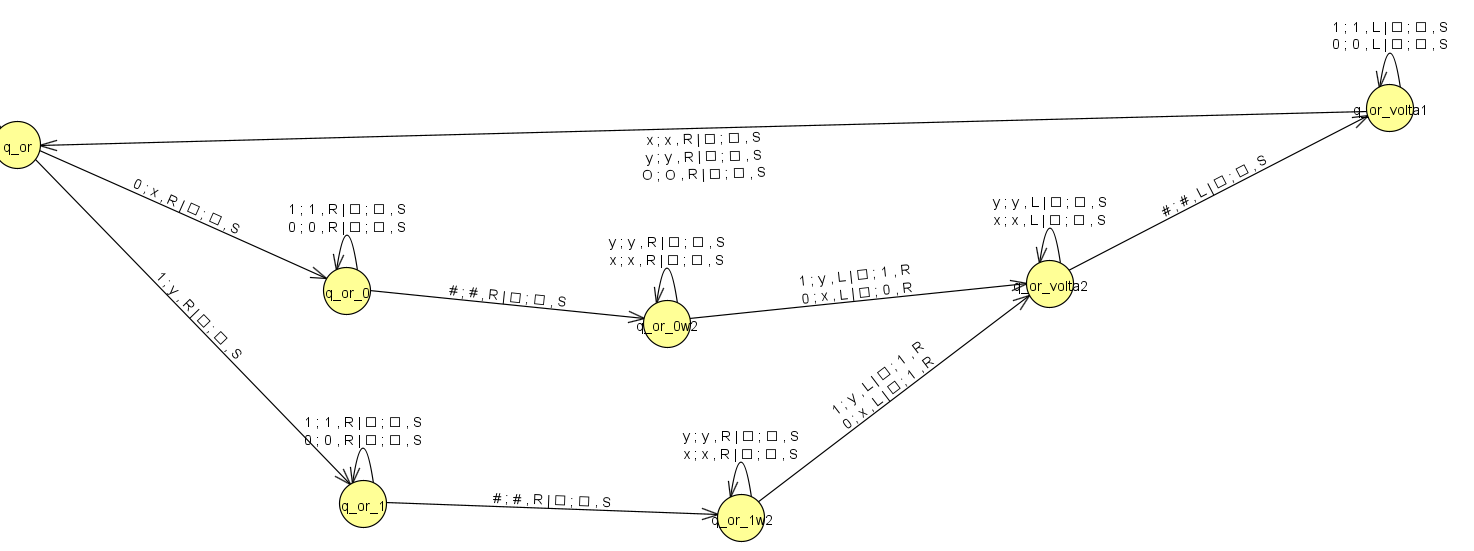
\includegraphics[width=\linewidth,height=0.22\textheight,keepaspectratio]{figuras/diagramas/diag_or.png}\\[0.2em]
{\small (b) Bloco OR}\\[0.8em]
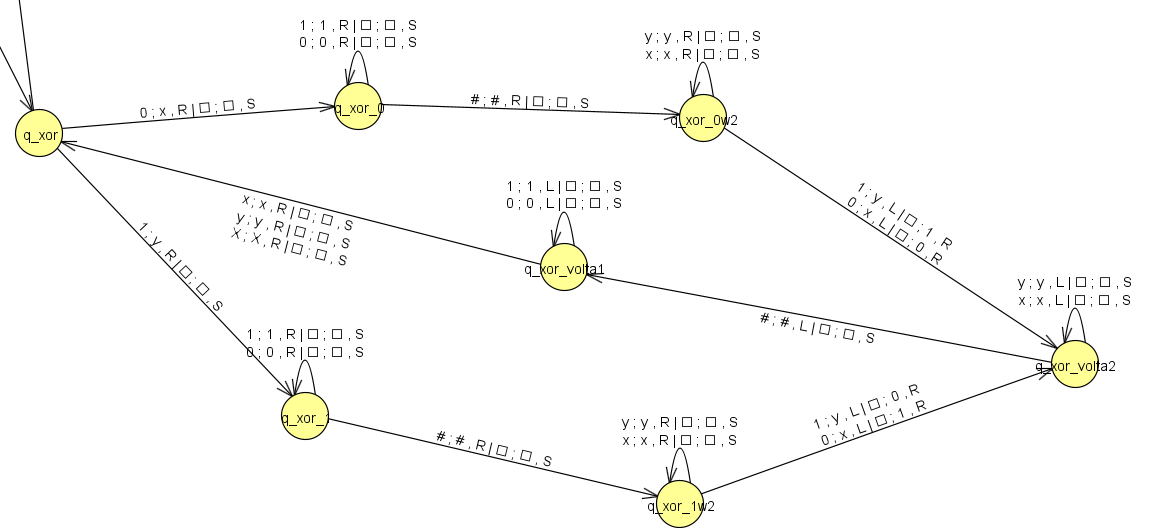
\includegraphics[width=\linewidth,height=0.22\textheight,keepaspectratio]{figuras/diagramas/diag_xor.png}\\[0.2em]
{\small (c) Bloco XOR}
\caption{Ampliação de cada bloco de operação}
\label{fig:blocos}
\end{figure}

Os três blocos da Figura~\ref{fig:blocos} têm a mesma estrutura; mudam apenas os
bits escritos na fita 2 nas transições que saem de \s{q\_op\_0w2} e \s{q\_op\_1w2}.

% ======================================================================
\chapter{Implementação em Python}
\label{cap:implementacao}

\section{Estrutura do simulador}

O programa representa explicitamente os elementos da máquina:
\begin{itemize}
  \item fita 1 (\s{fita1}) e fita 2 (\s{fita2}), como listas de símbolos completadas
        com $B$ à direita conforme necessário;
  \item estado atual (\s{estado});
  \item posições das cabeças (\s{cabeca1} e \s{cabeca2});
  \item função de transição (\s{transicoes}), um dicionário que associa cada
        tripla $(q, X_1, X_2)$ à quíntupla $(p, Y_1, Y_2, D_1, D_2)$.
\end{itemize}

O laço do simulador apenas lê os dois símbolos sob as cabeças, procura a transição
em $\delta$, escreve, move as cabeças e troca de estado. Não há nenhum operador
lógico do Python (\s{and}, \s{or}, \s{\textasciicircum}, \s{\&}, \s{|}) aplicado aos
bits: os resultados estão nas entradas de $\delta$. A operação também não é informada
separadamente; o programa recebe apenas a cadeia (por exemplo, \s{X101\#110}).

\section{Execução}

O comando \s{python3 mt\_duas\_fitas.py} executa todos os casos de teste; o comando
\s{python3 mt\_duas\_fitas.py X101\#110} executa uma entrada específica. A cada
passo, o programa mostra o estado atual, o conteúdo das duas fitas e a posição de
cada cabeça.

\section{Código-fonte}

O código-fonte completo também está disponível no repositório do GitHub:
\begin{center}
\textcolor{uftazul}{\url{https://github.com/matheuspontes01/MaquinaDeTuring}}
\end{center}

\lstinputlisting[language=Python, basicstyle=\ttfamily\scriptsize, columns=fullflexible, keepspaces=true, caption={Simulador da Máquina de Turing de duas fitas (\texttt{mt\_duas\_fitas.py})}, label={lst:codigo}]{mt_duas_fitas.py}

% ======================================================================
\chapter{Testes e Resultados}
\label{cap:testes}

\section{Casos de teste}

Foram executados 9 casos de teste (três por operação), com palavras de comprimento
1 a 5 e diferentes combinações de bits. A Tabela~\ref{tab:testes} resume os
resultados no formato entrada $\rightarrow$ resultado esperado $\rightarrow$
resultado obtido.

\begin{table}[H]
\centering
\caption{Resumo dos casos de teste}
\label{tab:testes}
\small
\begin{tabular}{llllc}
\toprule
\textbf{Entrada} & \textbf{Esperado} & \textbf{Obtido} & \textbf{Passos} & \textbf{Situação} \\
\midrule
\s{A0\#0}          & \s{0}     & \s{0}     & 13 & OK \\
\s{A101\#110}      & \s{100}   & \s{100}   & 41 & OK \\
\s{A11010\#10011}  & \s{10010} & \s{10010} & 85 & OK \\
\s{O01\#11}        & \s{11}    & \s{11}    & 25 & OK \\
\s{O101\#110}      & \s{111}   & \s{111}   & 41 & OK \\
\s{O0000\#0000}    & \s{0000}  & \s{0000}  & 61 & OK \\
\s{X01\#11}        & \s{10}    & \s{10}    & 25 & OK \\
\s{X101\#110}      & \s{011}   & \s{011}   & 41 & OK \\
\s{X1100\#1010}    & \s{0110}  & \s{0110}  & 61 & OK \\
\bottomrule
\end{tabular}
\end{table}

Todos os casos terminaram no estado \s{q\_aceita}, com a fita 2 contendo somente o
resultado e a fita 1 restaurada para a entrada original. A
Figura~\ref{fig:resumo} mostra a tela do resumo da execução.

\begin{figure}[H]
\centering
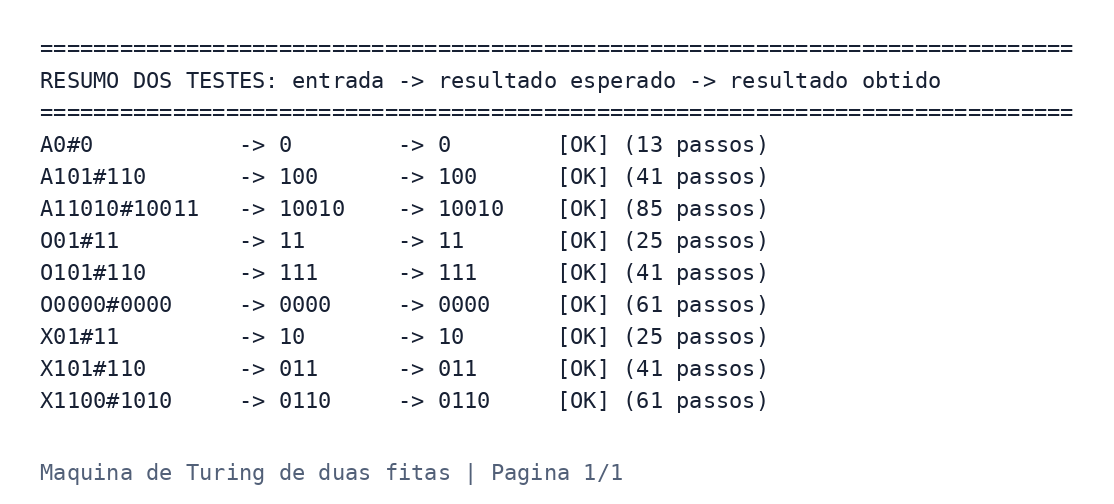
\includegraphics[width=\linewidth]{figuras/resumo.png}
\caption{Resumo da execução dos testes}
\label{fig:resumo}
\end{figure}

\section{Execução passo a passo}

Nas telas a seguir, cada passo mostra o estado atual, o conteúdo da fita 1 e da
fita 2 e as posições das duas cabeças. A célula sob cada cabeça aparece entre
colchetes.

% ── Teste 1: A0#0 → 0 ─────────────────────────────────────────────
\subsection{Teste 1: \texttt{A0\#0}}
\label{sec:teste1}

\begin{figure}[H]
\centering
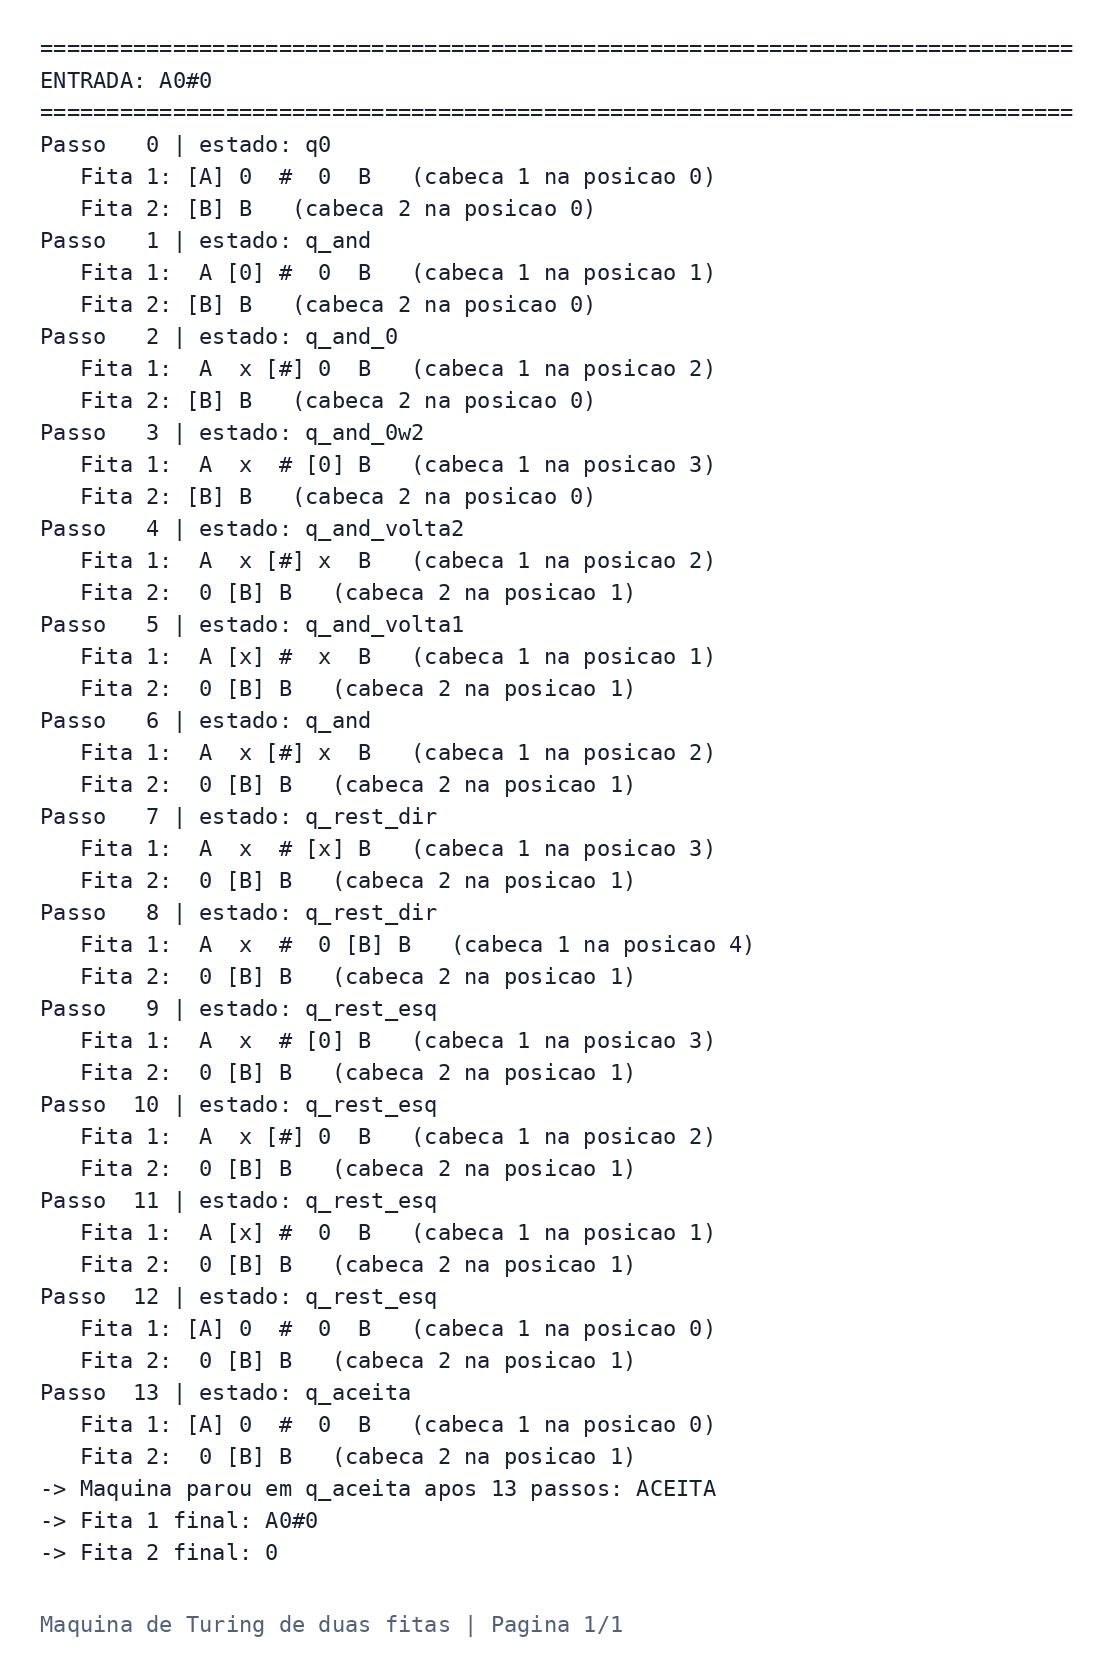
\includegraphics[width=\linewidth,height=0.78\textheight,keepaspectratio]{figuras/execucao/teste1_01.png}
\caption{Execução passo a passo da entrada \texttt{A0\#0} (esperado: \texttt{0})}
\end{figure}

% ── Teste 2: A101#110 → 100 ───────────────────────────────────────
\subsection{Teste 2: \texttt{A101\#110}}
\label{sec:teste2}

\begin{figure}[H]
\centering
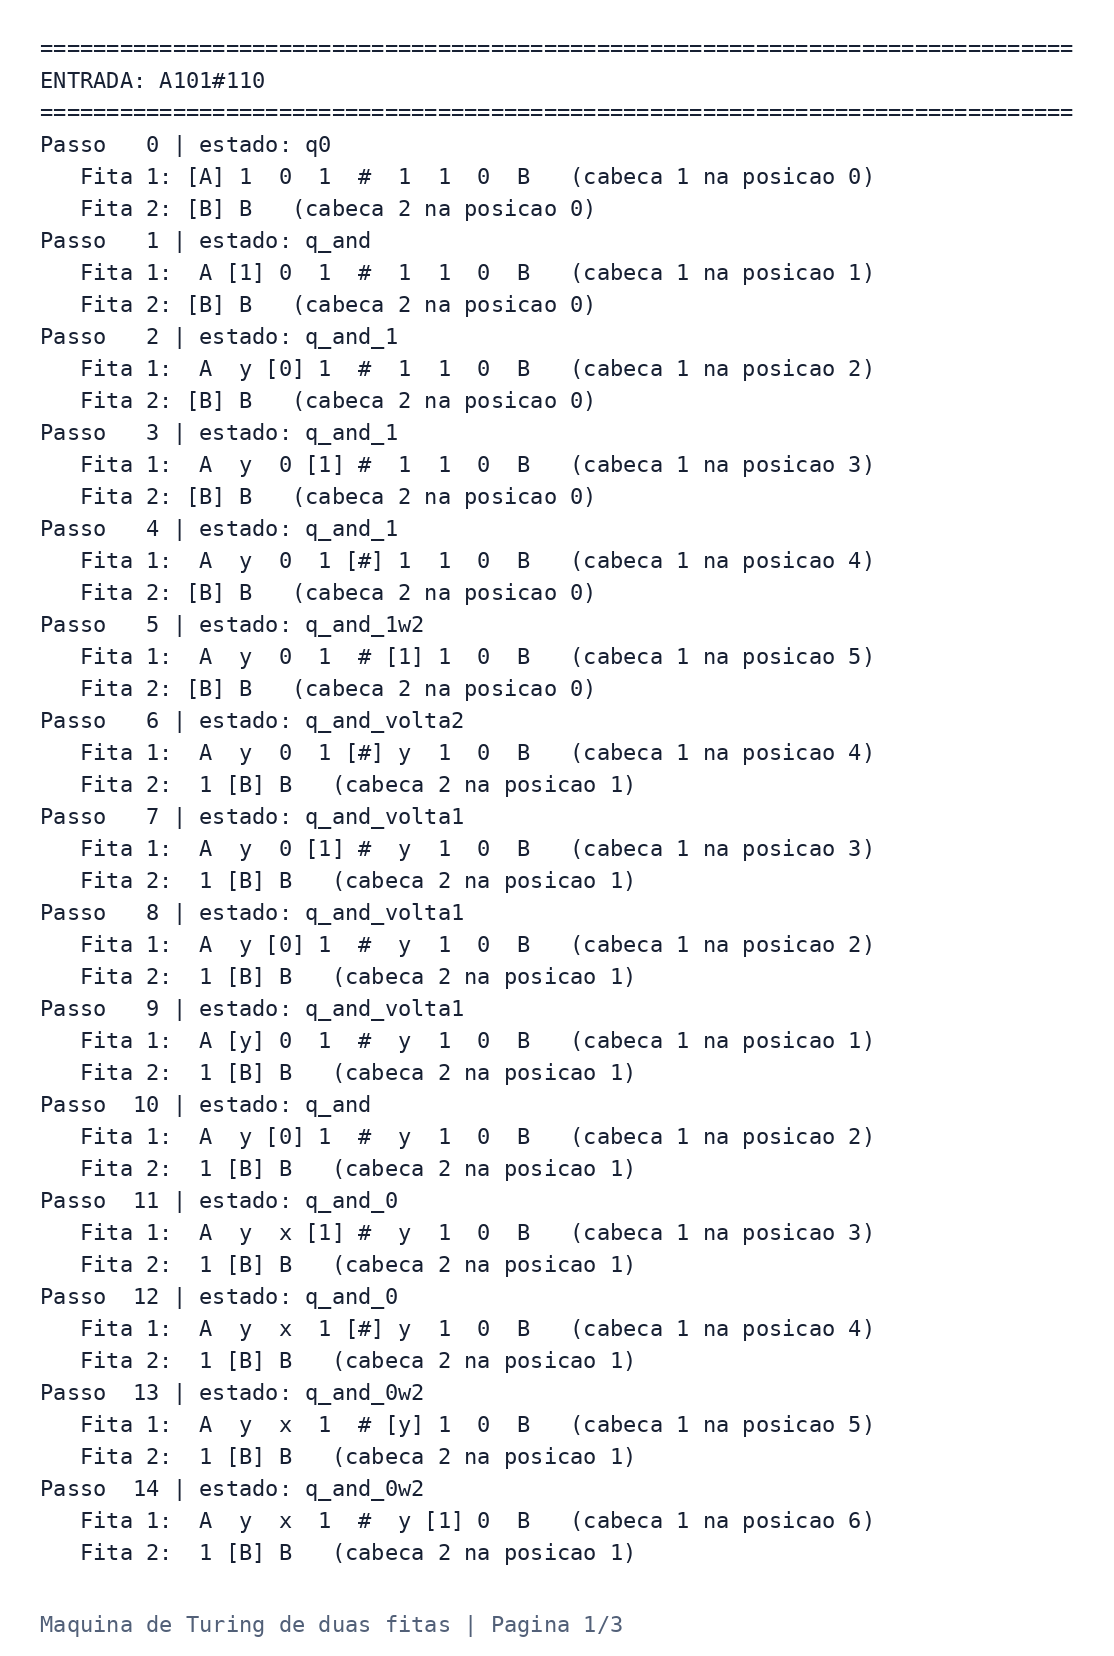
\includegraphics[width=\linewidth,height=0.78\textheight,keepaspectratio]{figuras/execucao/teste2_01.png}
\caption{Execução passo a passo da entrada \texttt{A101\#110} (esperado: \texttt{100}) --- parte 1 de 3}
\end{figure}

\begin{figure}[H]
\centering
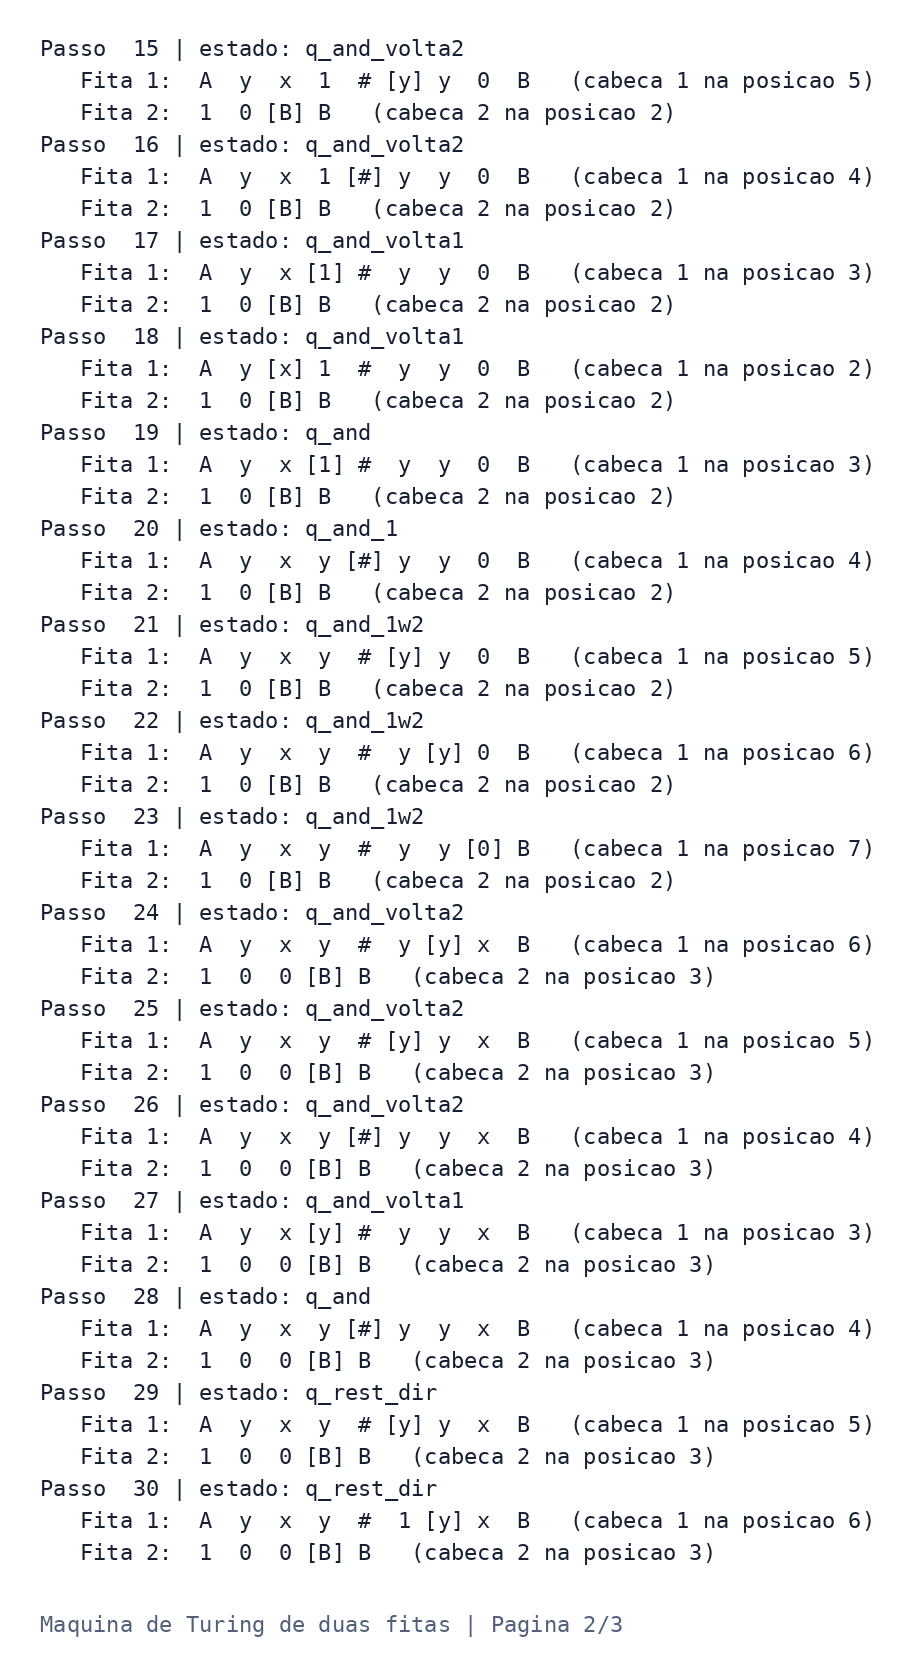
\includegraphics[width=\linewidth,height=0.78\textheight,keepaspectratio]{figuras/execucao/teste2_02.png}
\caption{Execução passo a passo da entrada \texttt{A101\#110} (esperado: \texttt{100}) --- parte 2 de 3}
\end{figure}

\begin{figure}[H]
\centering
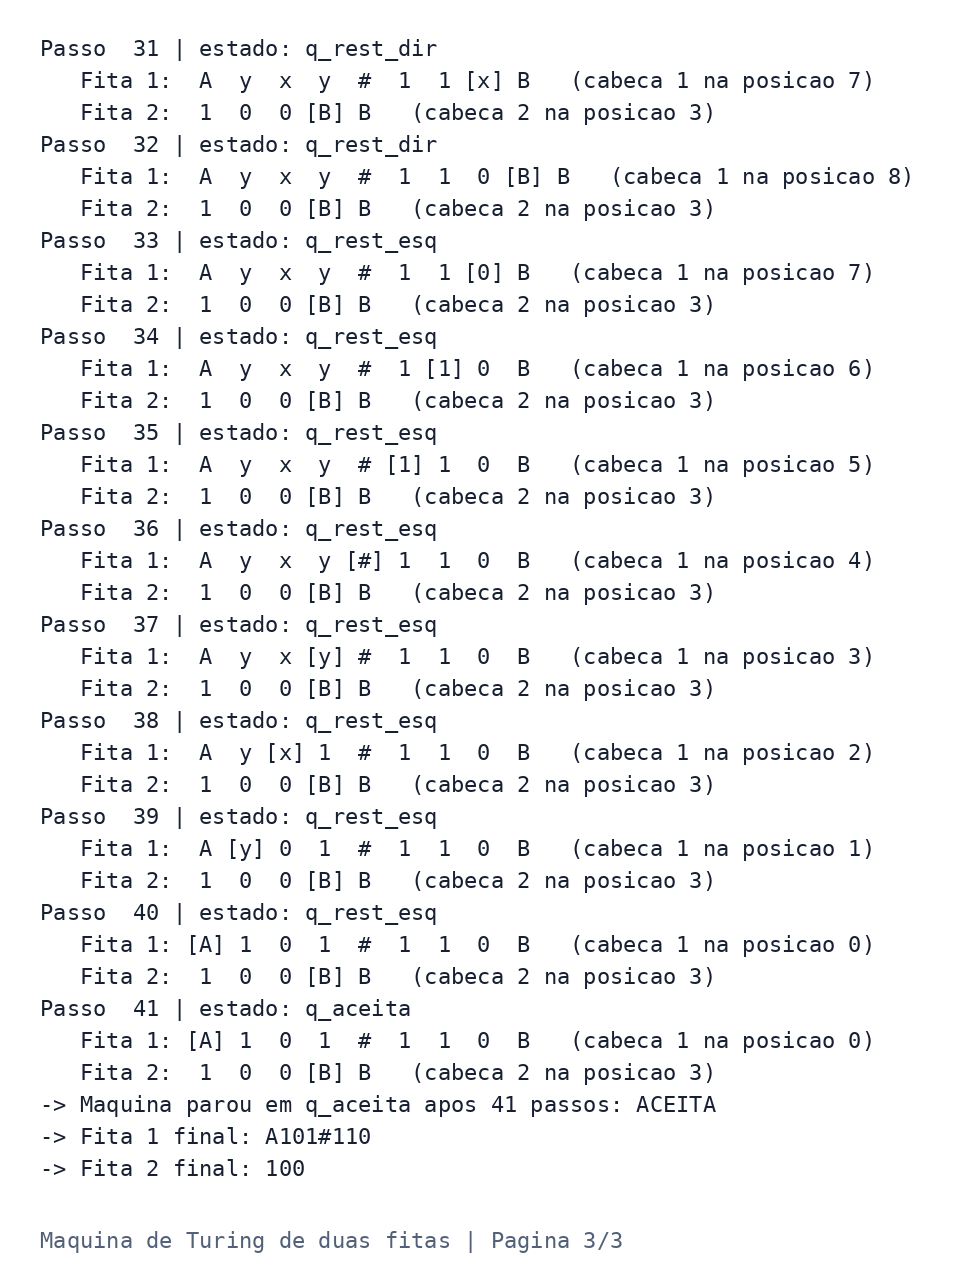
\includegraphics[width=\linewidth,height=0.78\textheight,keepaspectratio]{figuras/execucao/teste2_03.png}
\caption{Execução passo a passo da entrada \texttt{A101\#110} (esperado: \texttt{100}) --- parte 3 de 3}
\end{figure}

% ── Teste 3: A11010#10011 → 10010 ─────────────────────────────────
\subsection{Teste 3: \texttt{A11010\#10011}}
\label{sec:teste3}

\begin{figure}[H]
\centering
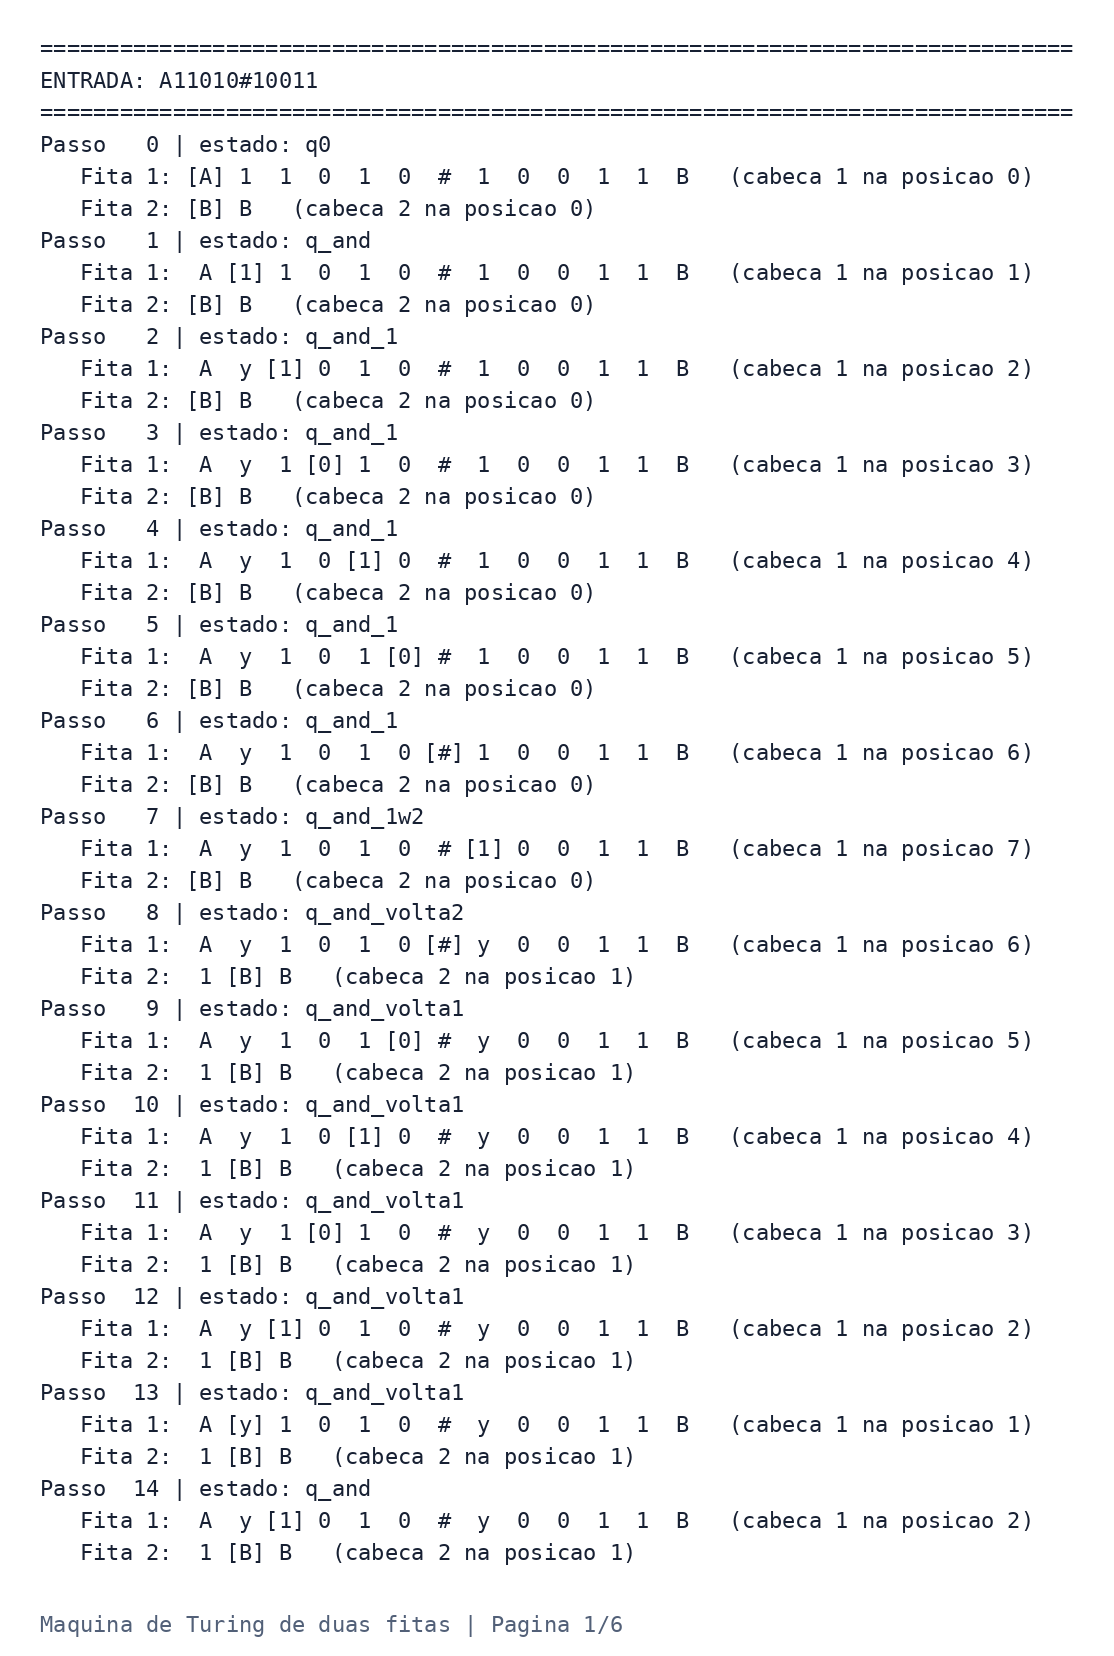
\includegraphics[width=\linewidth,height=0.78\textheight,keepaspectratio]{figuras/execucao/teste3_01.png}
\caption{Execução passo a passo da entrada \texttt{A11010\#10011} (esperado: \texttt{10010}) --- parte 1 de 6}
\end{figure}

\begin{figure}[H]
\centering
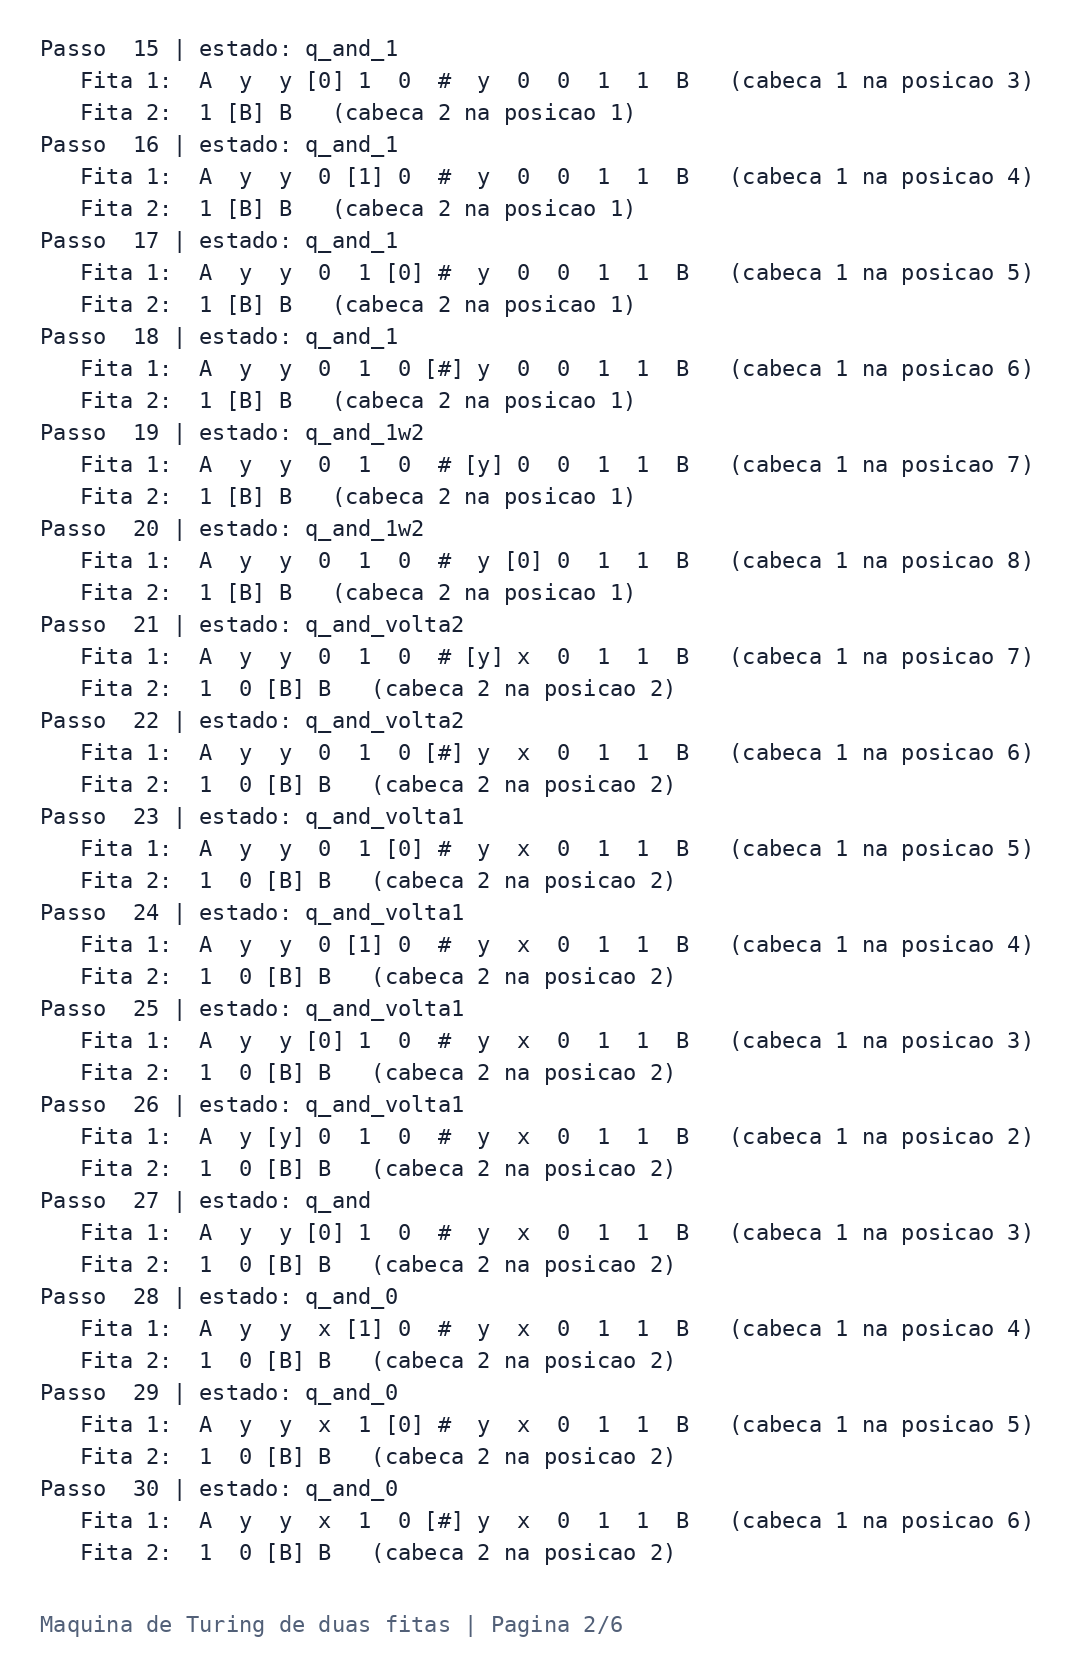
\includegraphics[width=\linewidth,height=0.78\textheight,keepaspectratio]{figuras/execucao/teste3_02.png}
\caption{Execução passo a passo da entrada \texttt{A11010\#10011} (esperado: \texttt{10010}) --- parte 2 de 6}
\end{figure}

\begin{figure}[H]
\centering
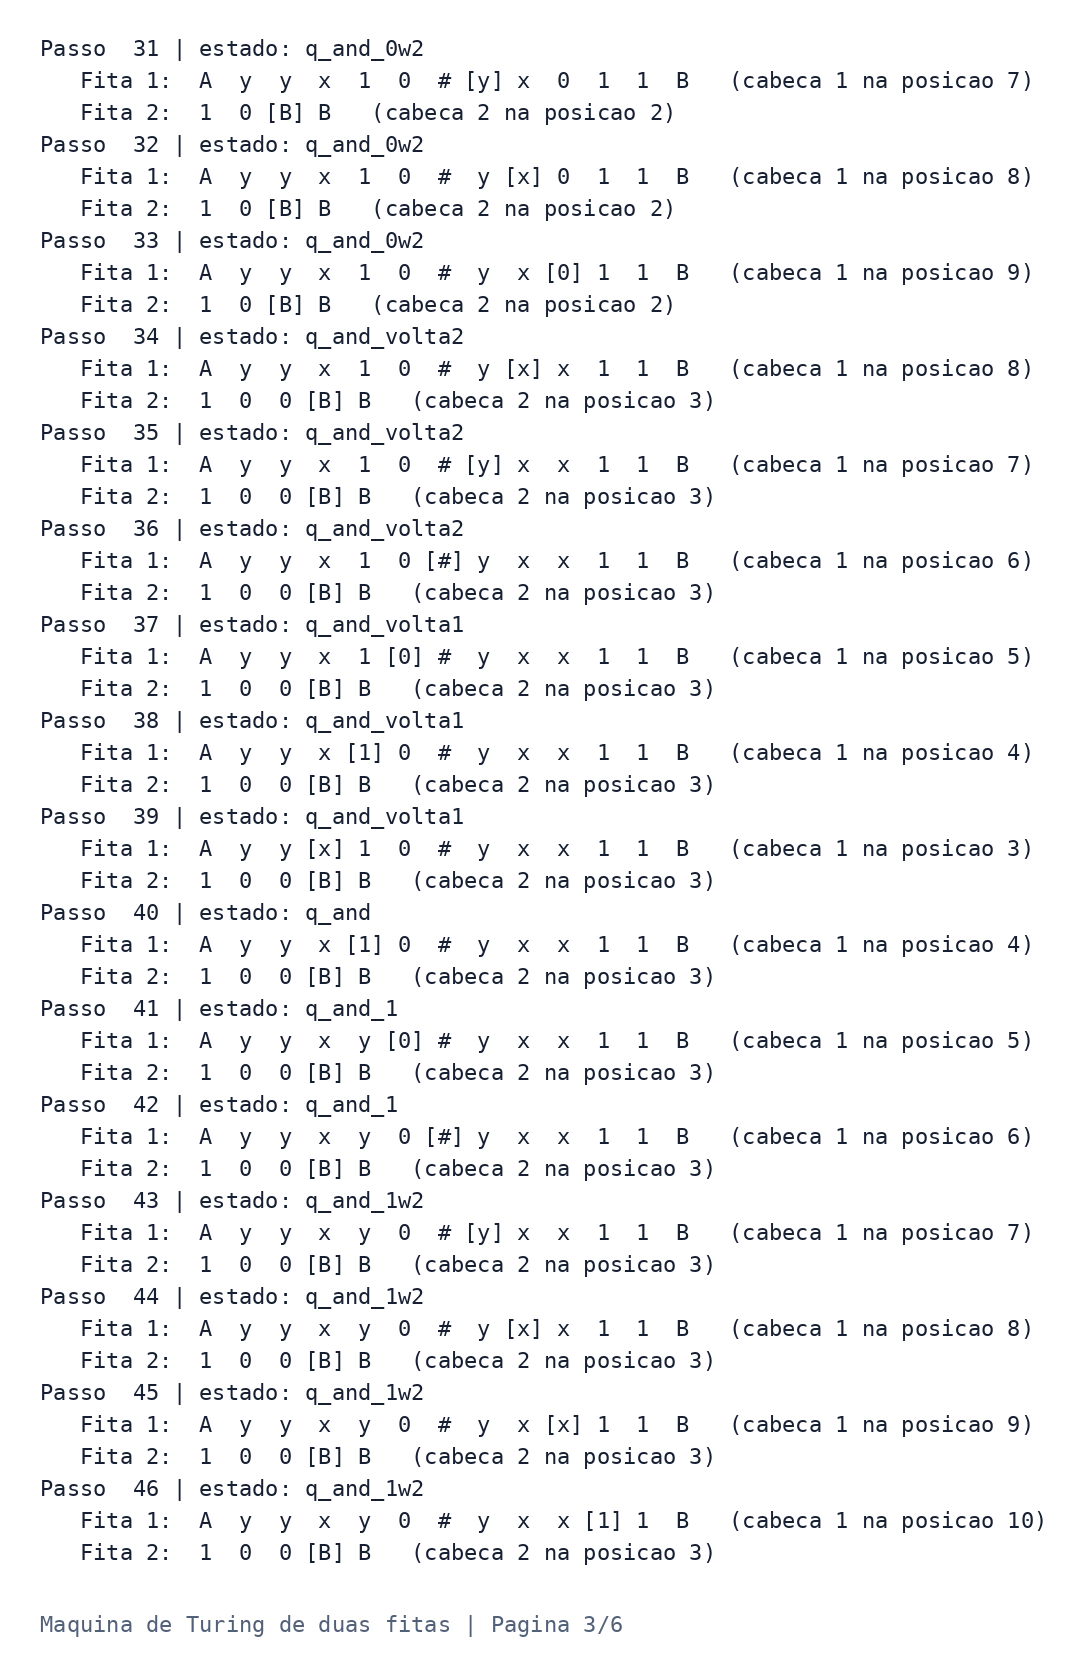
\includegraphics[width=\linewidth,height=0.78\textheight,keepaspectratio]{figuras/execucao/teste3_03.png}
\caption{Execução passo a passo da entrada \texttt{A11010\#10011} (esperado: \texttt{10010}) --- parte 3 de 6}
\end{figure}

\begin{figure}[H]
\centering
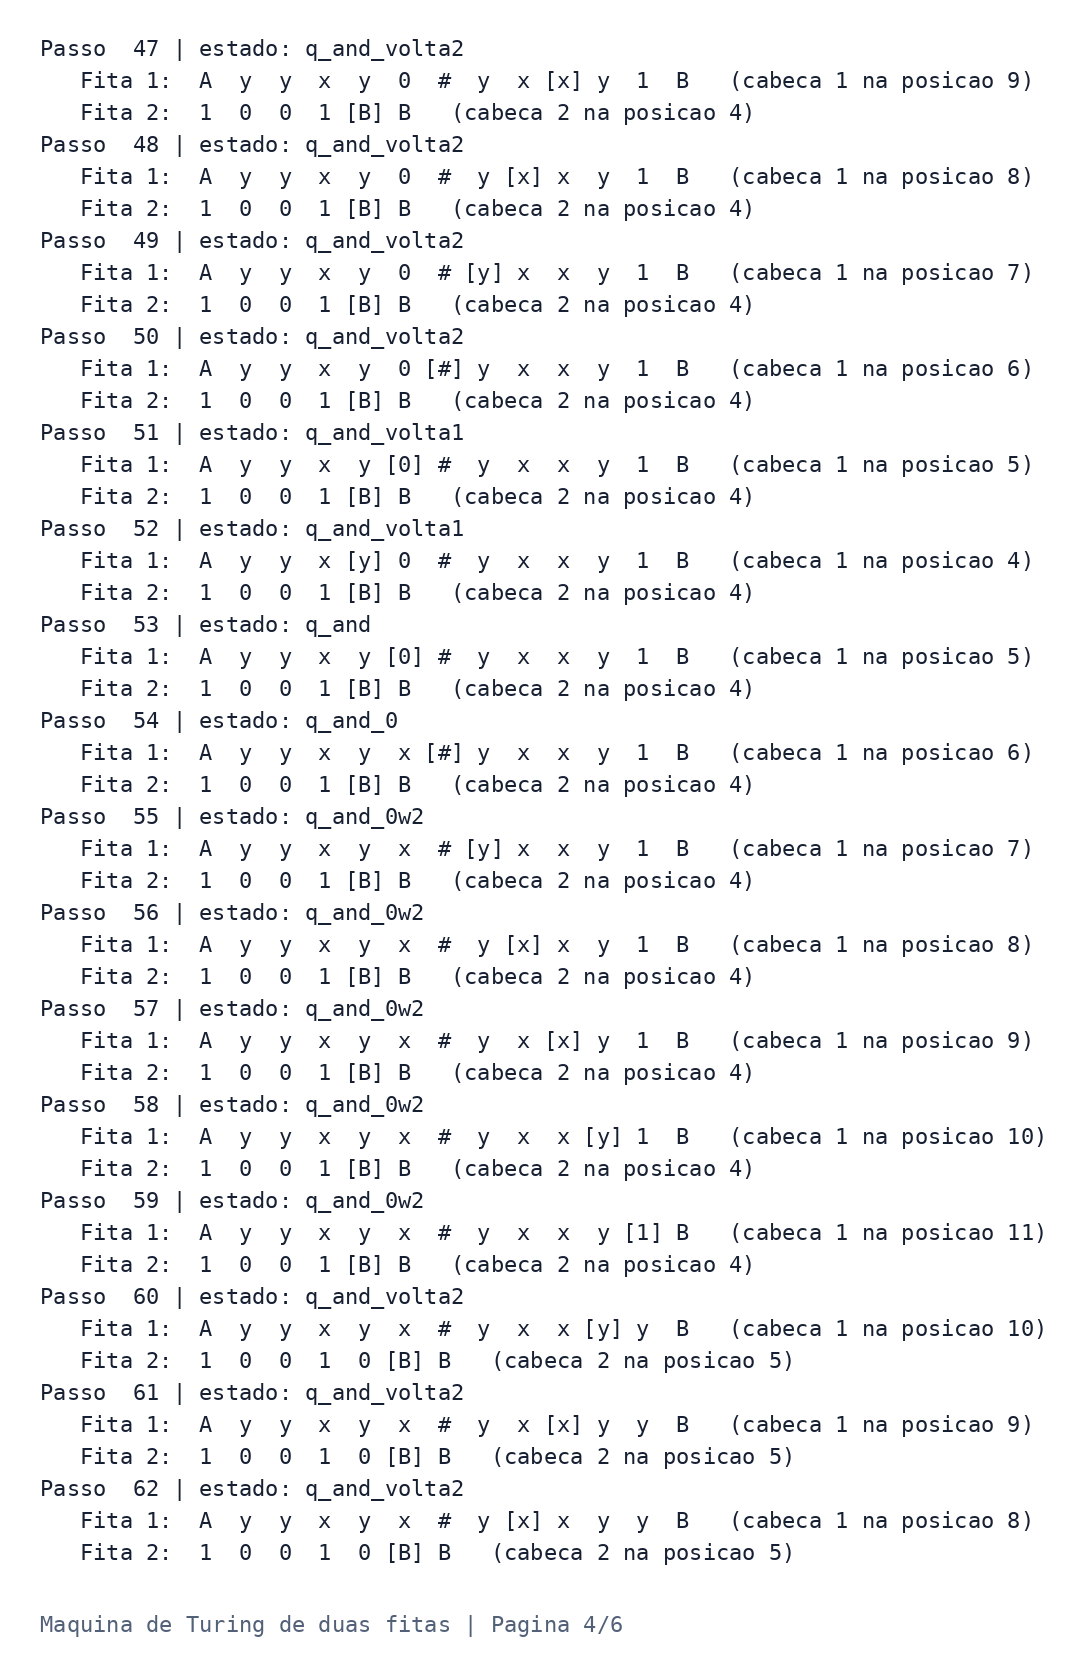
\includegraphics[width=\linewidth,height=0.78\textheight,keepaspectratio]{figuras/execucao/teste3_04.png}
\caption{Execução passo a passo da entrada \texttt{A11010\#10011} (esperado: \texttt{10010}) --- parte 4 de 6}
\end{figure}

\begin{figure}[H]
\centering
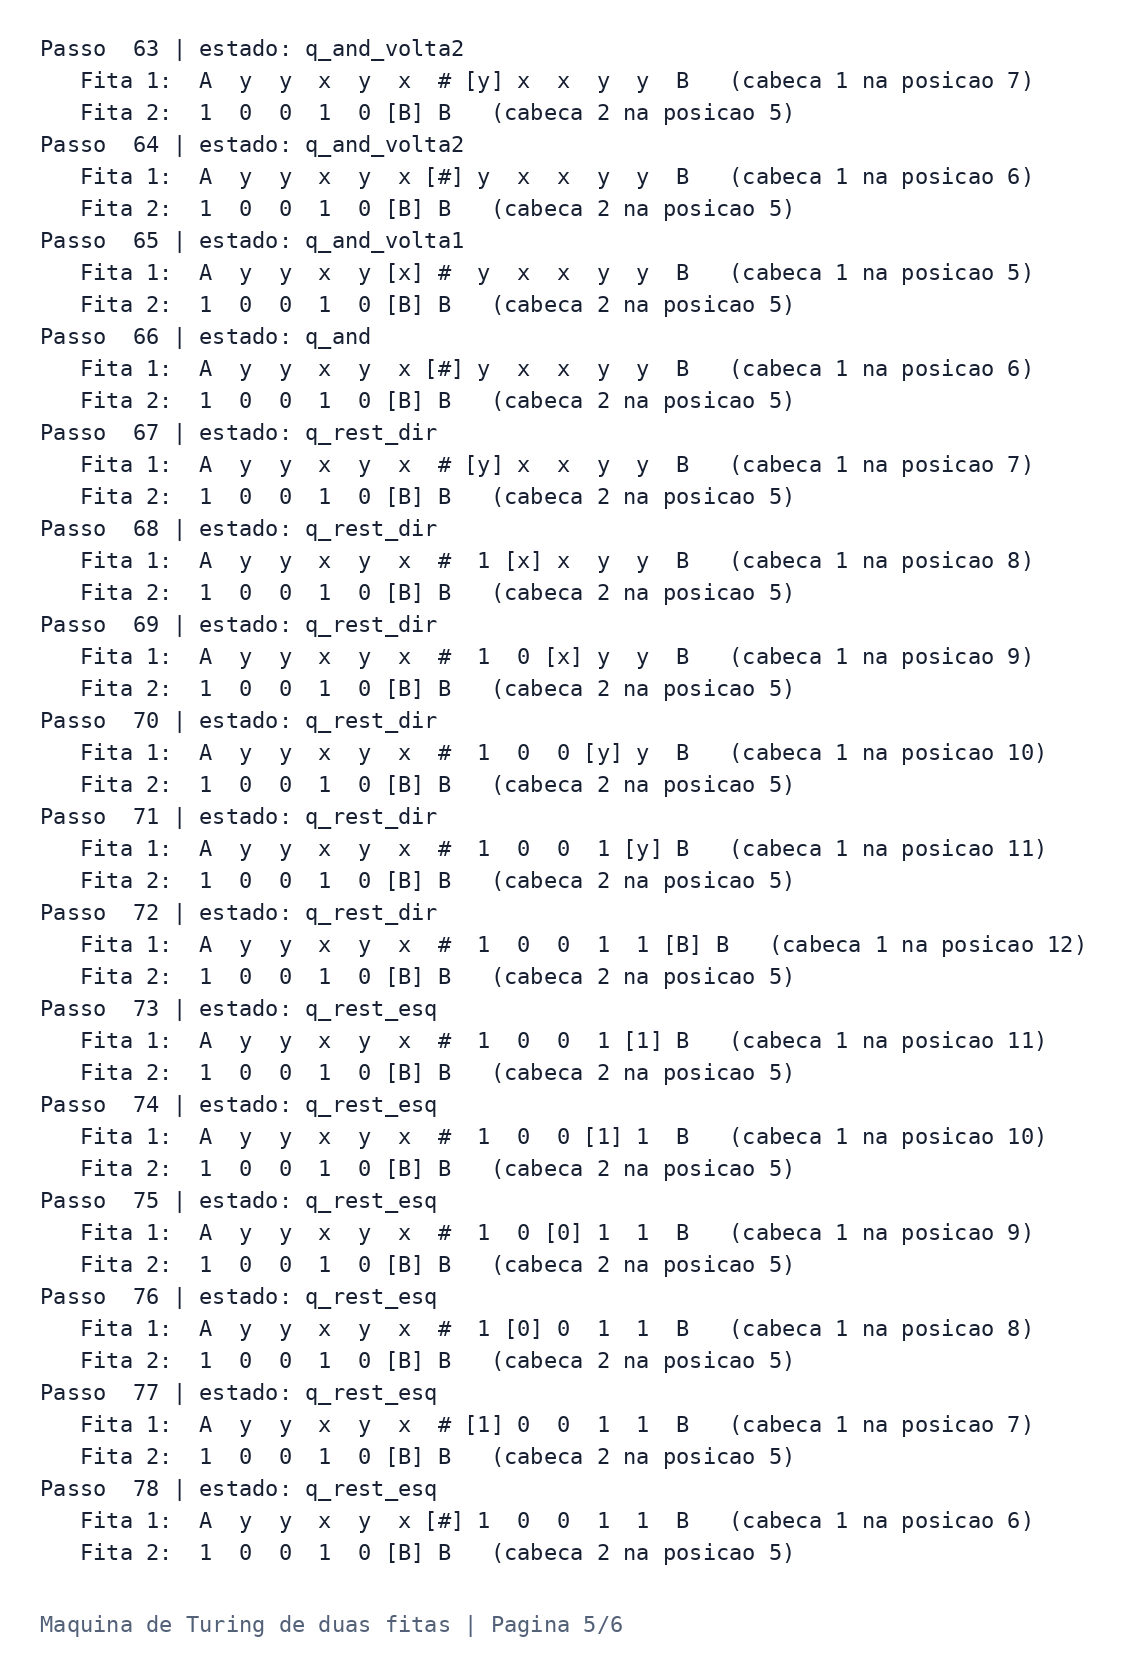
\includegraphics[width=\linewidth,height=0.78\textheight,keepaspectratio]{figuras/execucao/teste3_05.png}
\caption{Execução passo a passo da entrada \texttt{A11010\#10011} (esperado: \texttt{10010}) --- parte 5 de 6}
\end{figure}

\begin{figure}[H]
\centering
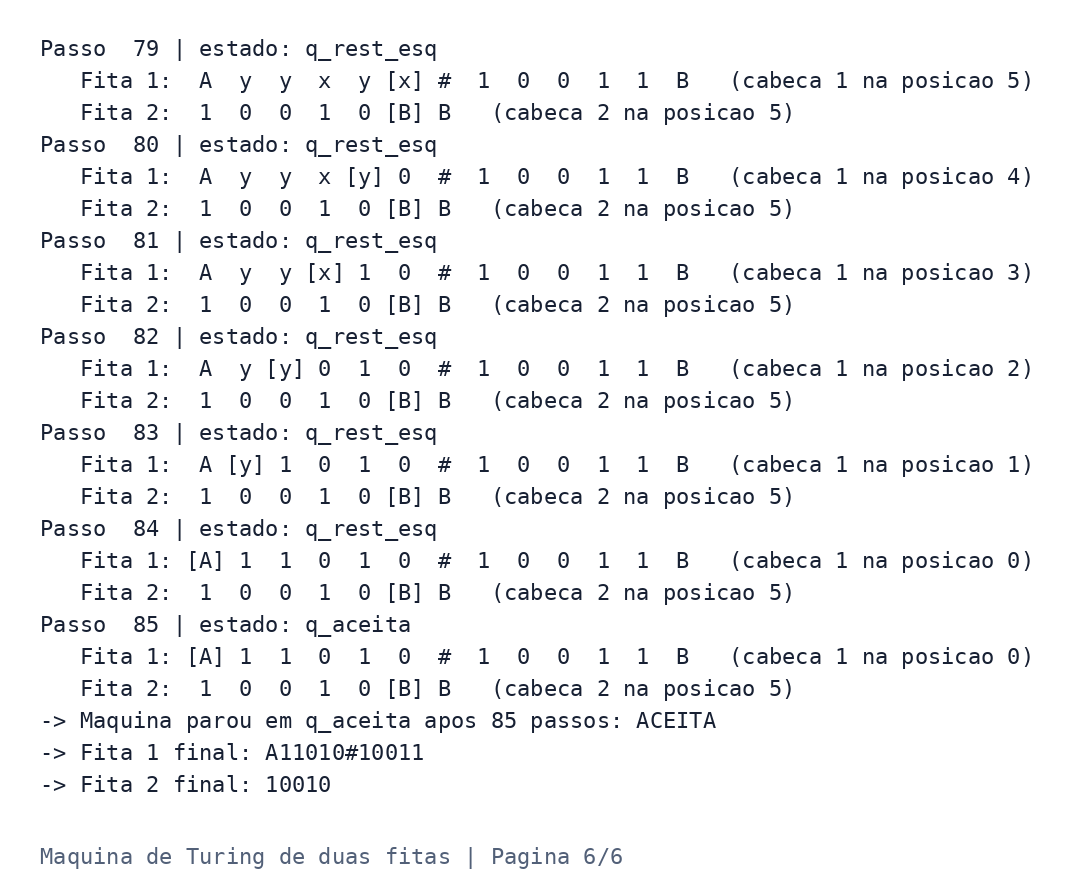
\includegraphics[width=\linewidth,height=0.78\textheight,keepaspectratio]{figuras/execucao/teste3_06.png}
\caption{Execução passo a passo da entrada \texttt{A11010\#10011} (esperado: \texttt{10010}) --- parte 6 de 6}
\end{figure}

% ── Teste 4: O01#11 → 11 ──────────────────────────────────────────
\subsection{Teste 4: \texttt{O01\#11}}
\label{sec:teste4}

\begin{figure}[H]
\centering
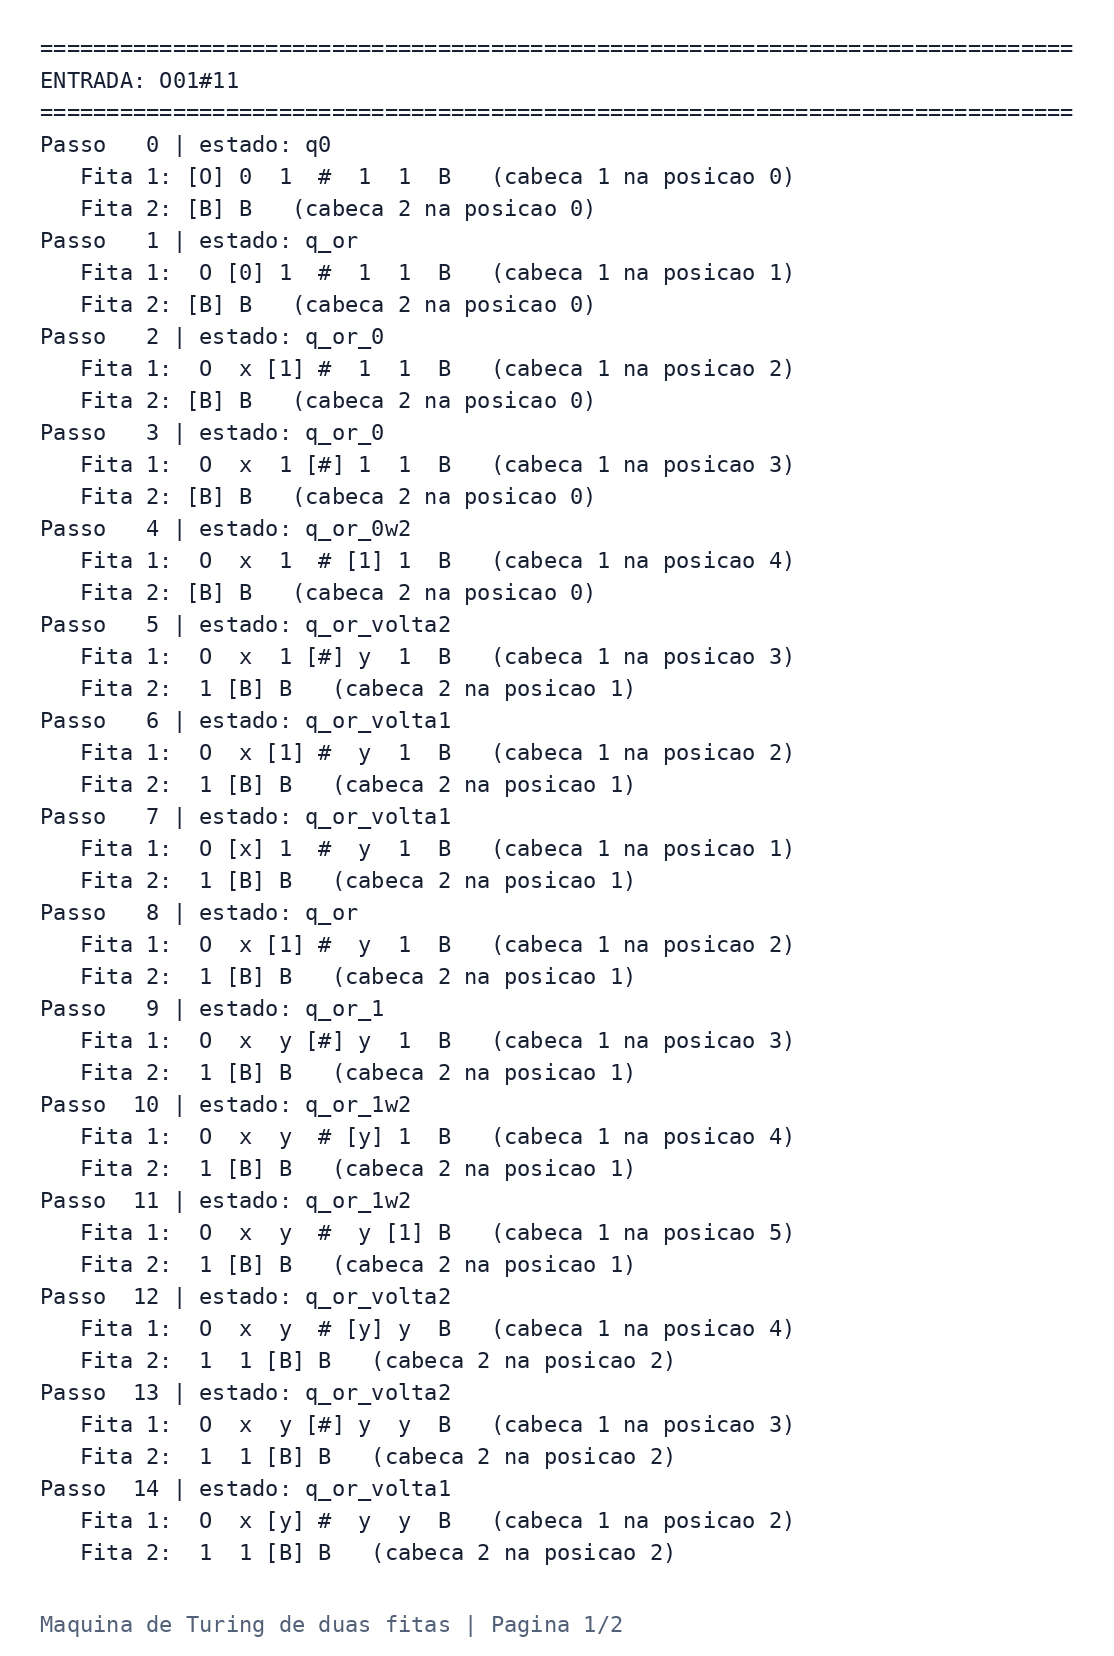
\includegraphics[width=\linewidth,height=0.78\textheight,keepaspectratio]{figuras/execucao/teste4_01.png}
\caption{Execução passo a passo da entrada \texttt{O01\#11} (esperado: \texttt{11}) --- parte 1 de 2}
\end{figure}

\begin{figure}[H]
\centering
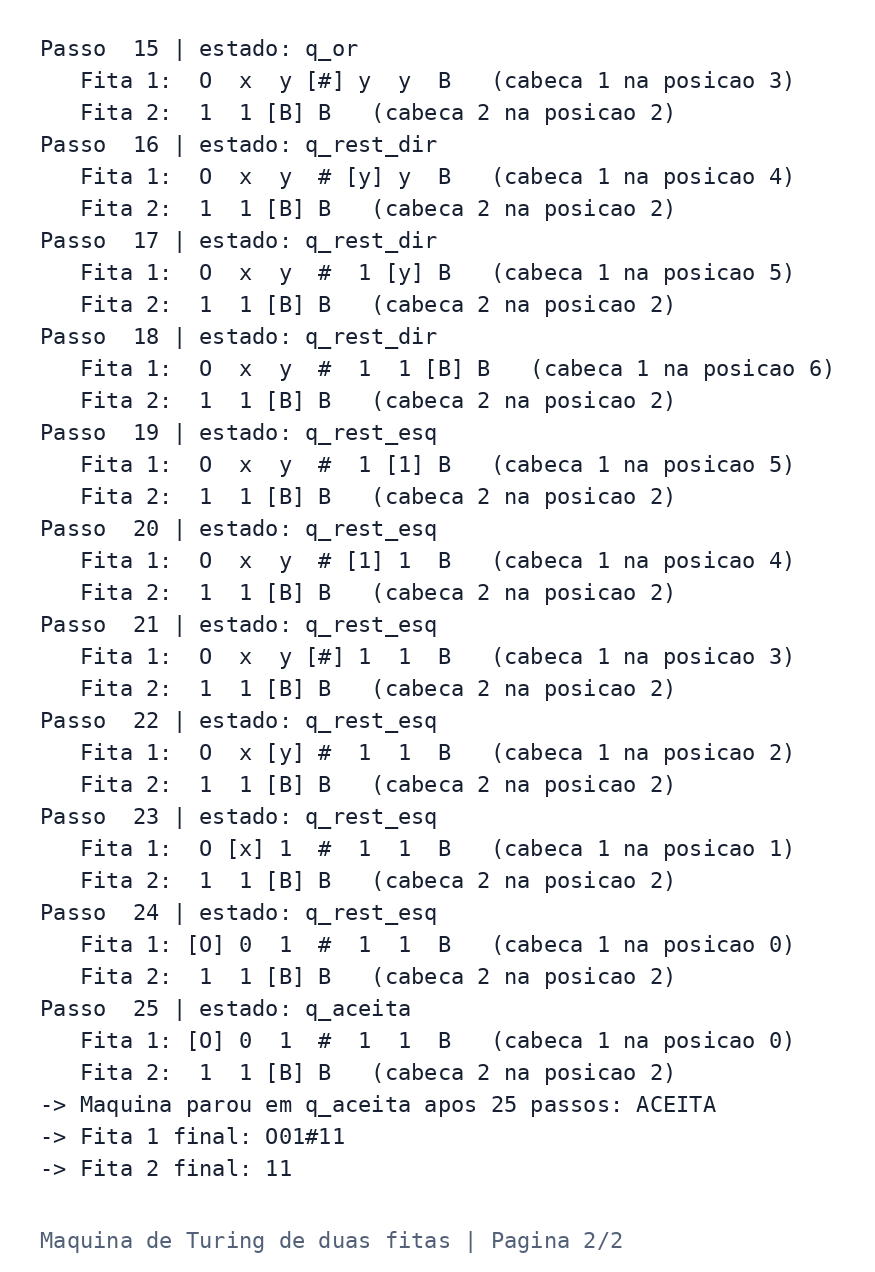
\includegraphics[width=\linewidth,height=0.78\textheight,keepaspectratio]{figuras/execucao/teste4_02.png}
\caption{Execução passo a passo da entrada \texttt{O01\#11} (esperado: \texttt{11}) --- parte 2 de 2}
\end{figure}

% ── Teste 5: O101#110 → 111 ───────────────────────────────────────
\subsection{Teste 5: \texttt{O101\#110}}
\label{sec:teste5}

\begin{figure}[H]
\centering
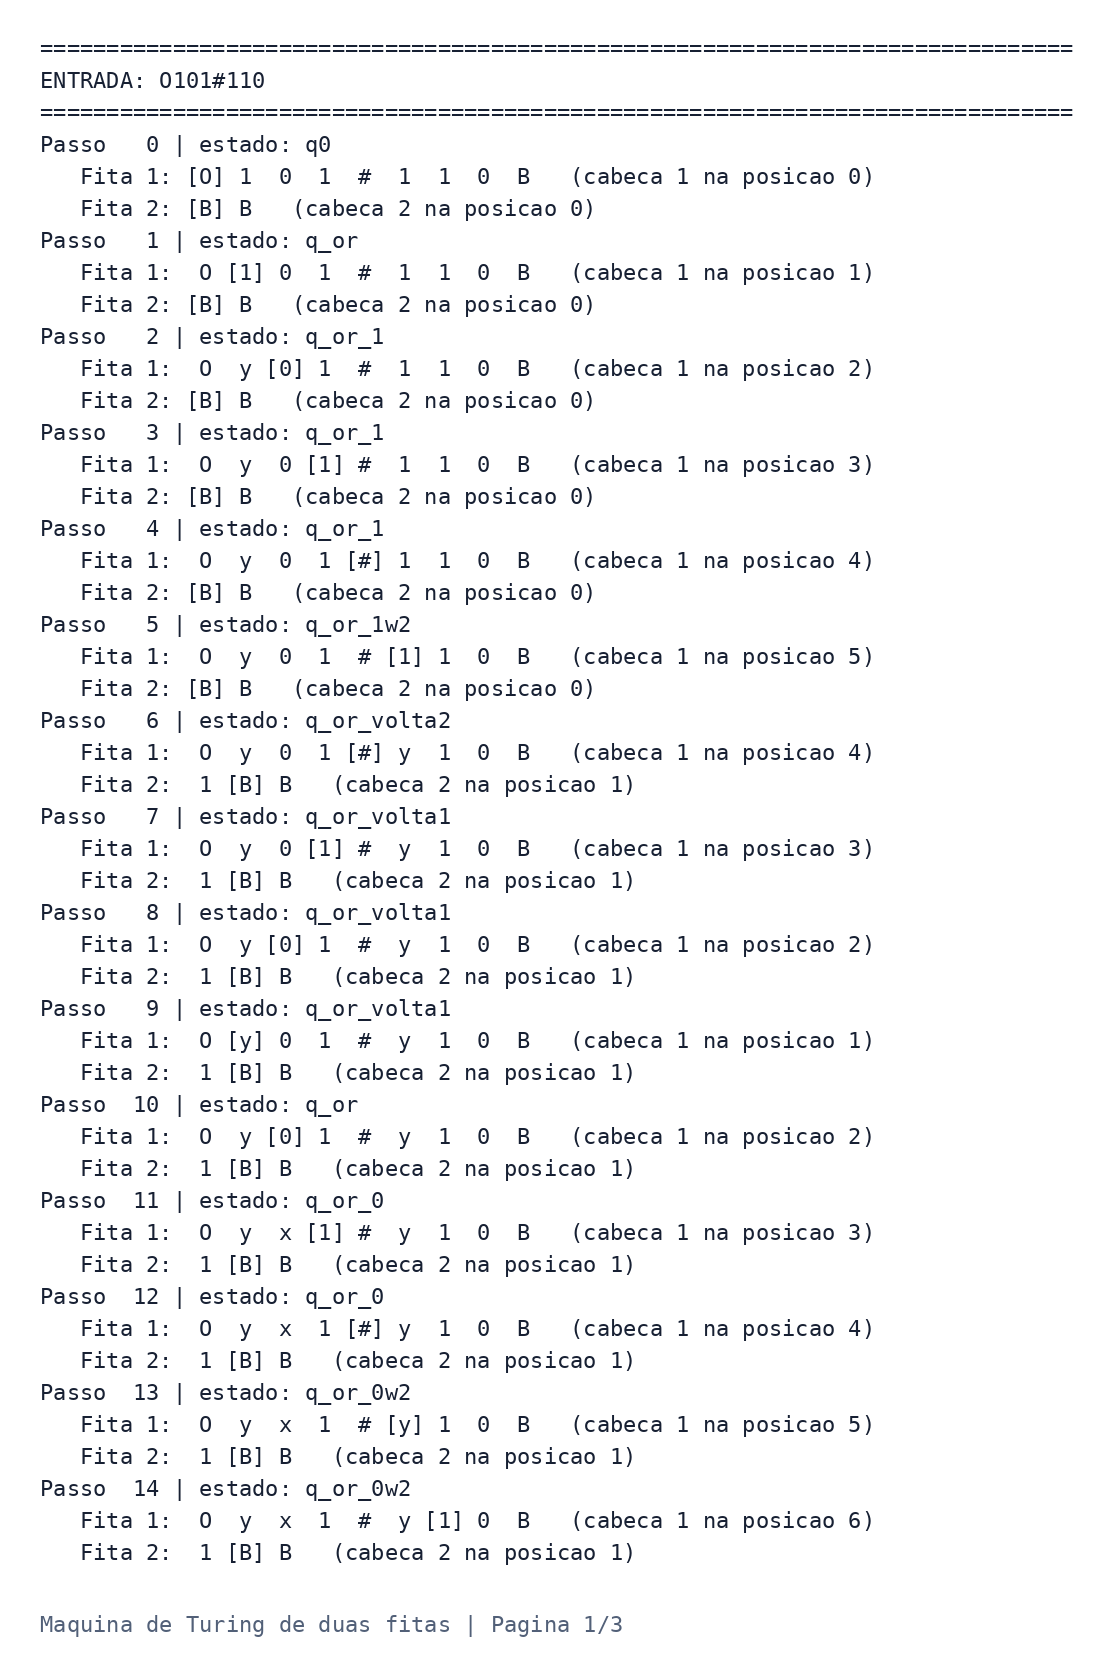
\includegraphics[width=\linewidth,height=0.78\textheight,keepaspectratio]{figuras/execucao/teste5_01.png}
\caption{Execução passo a passo da entrada \texttt{O101\#110} (esperado: \texttt{111}) --- parte 1 de 3}
\end{figure}

\begin{figure}[H]
\centering
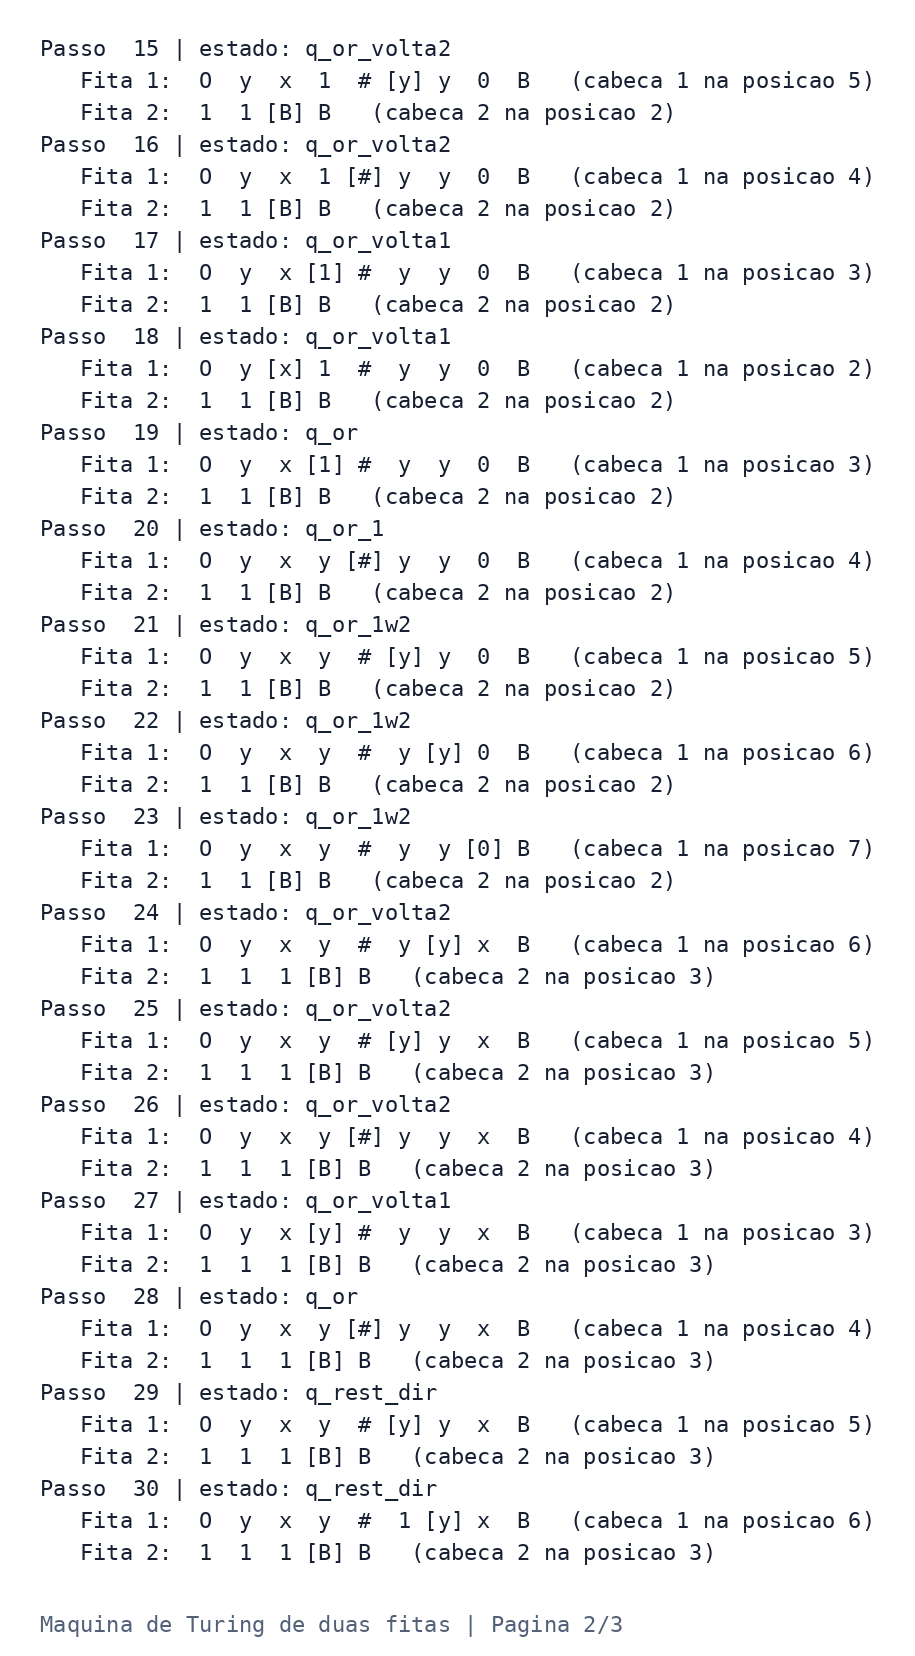
\includegraphics[width=\linewidth,height=0.78\textheight,keepaspectratio]{figuras/execucao/teste5_02.png}
\caption{Execução passo a passo da entrada \texttt{O101\#110} (esperado: \texttt{111}) --- parte 2 de 3}
\end{figure}

\begin{figure}[H]
\centering
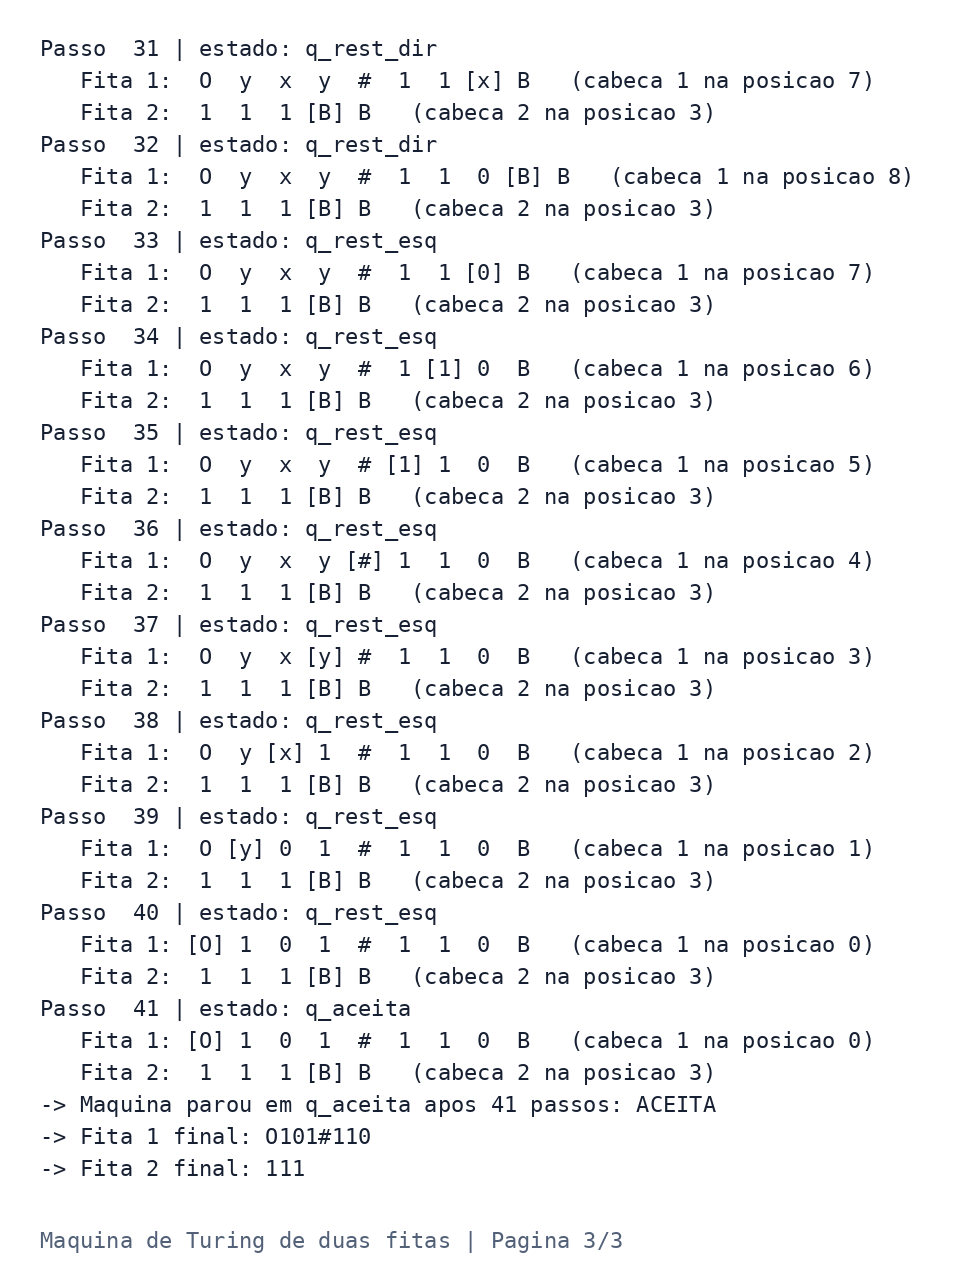
\includegraphics[width=\linewidth,height=0.78\textheight,keepaspectratio]{figuras/execucao/teste5_03.png}
\caption{Execução passo a passo da entrada \texttt{O101\#110} (esperado: \texttt{111}) --- parte 3 de 3}
\end{figure}

% ── Teste 6: O0000#0000 → 0000 ────────────────────────────────────
\subsection{Teste 6: \texttt{O0000\#0000}}
\label{sec:teste6}

\begin{figure}[H]
\centering
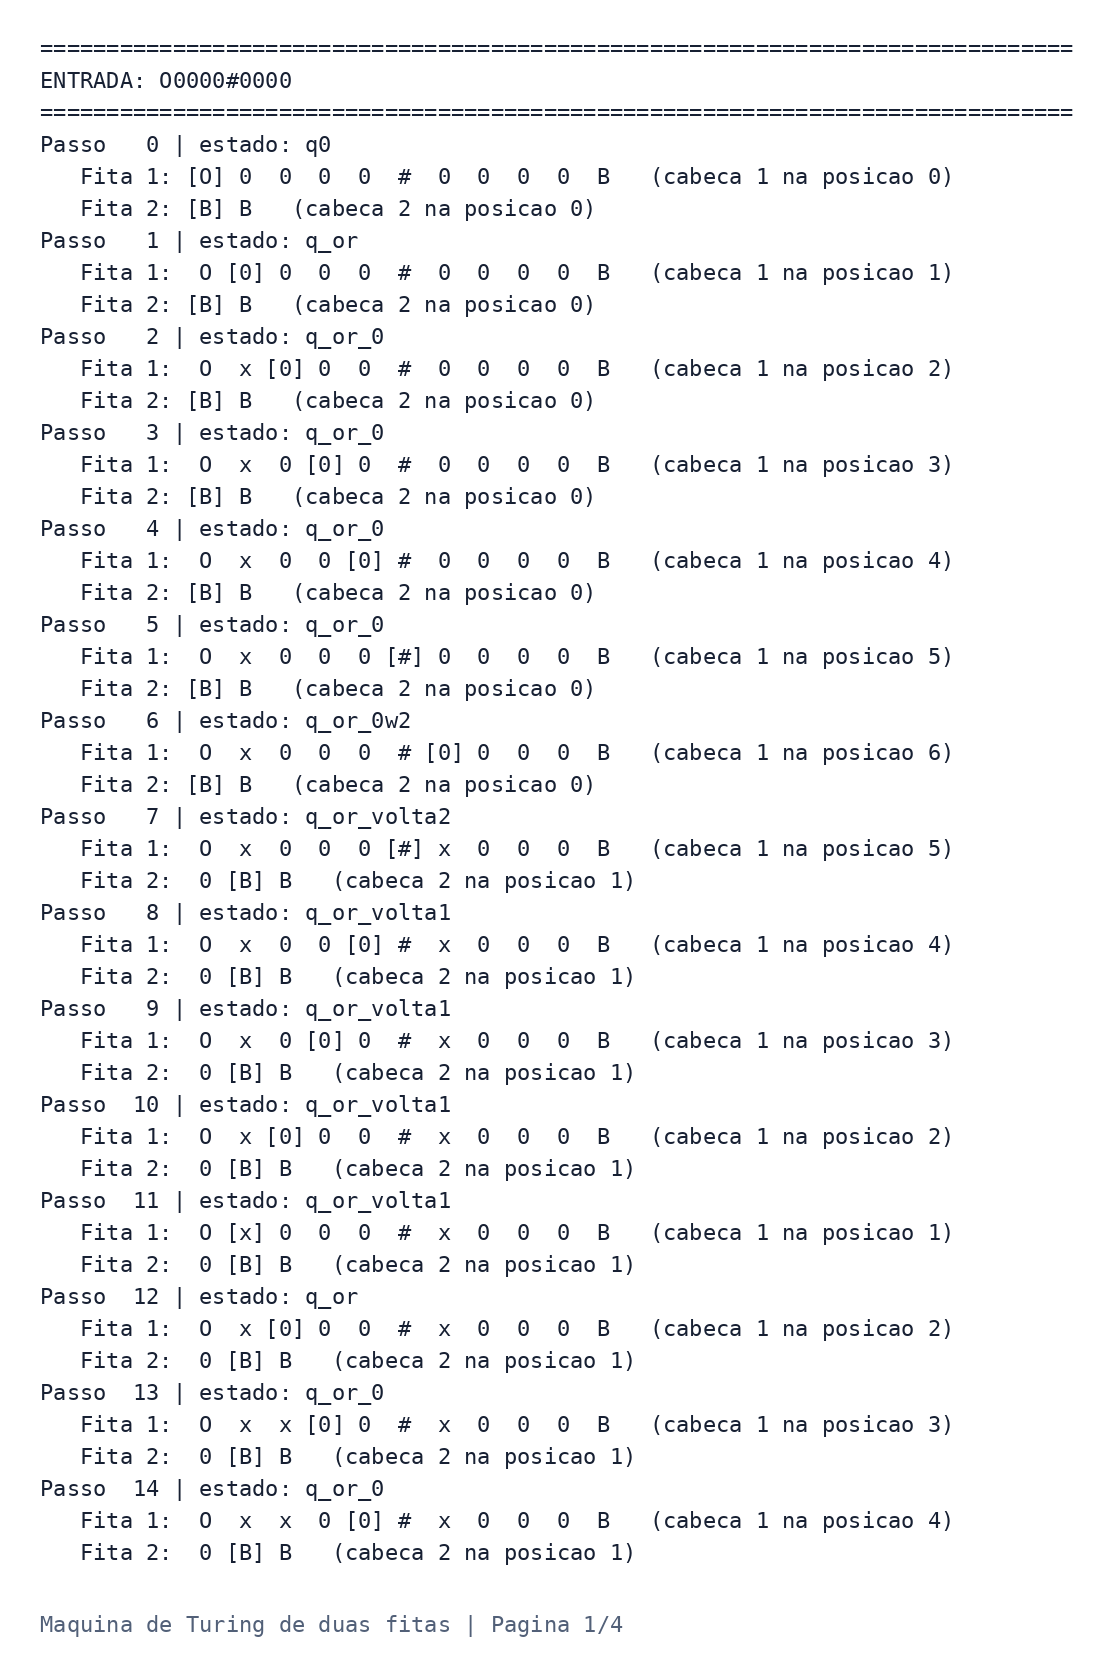
\includegraphics[width=\linewidth,height=0.78\textheight,keepaspectratio]{figuras/execucao/teste6_01.png}
\caption{Execução passo a passo da entrada \texttt{O0000\#0000} (esperado: \texttt{0000}) --- parte 1 de 4}
\end{figure}

\begin{figure}[H]
\centering
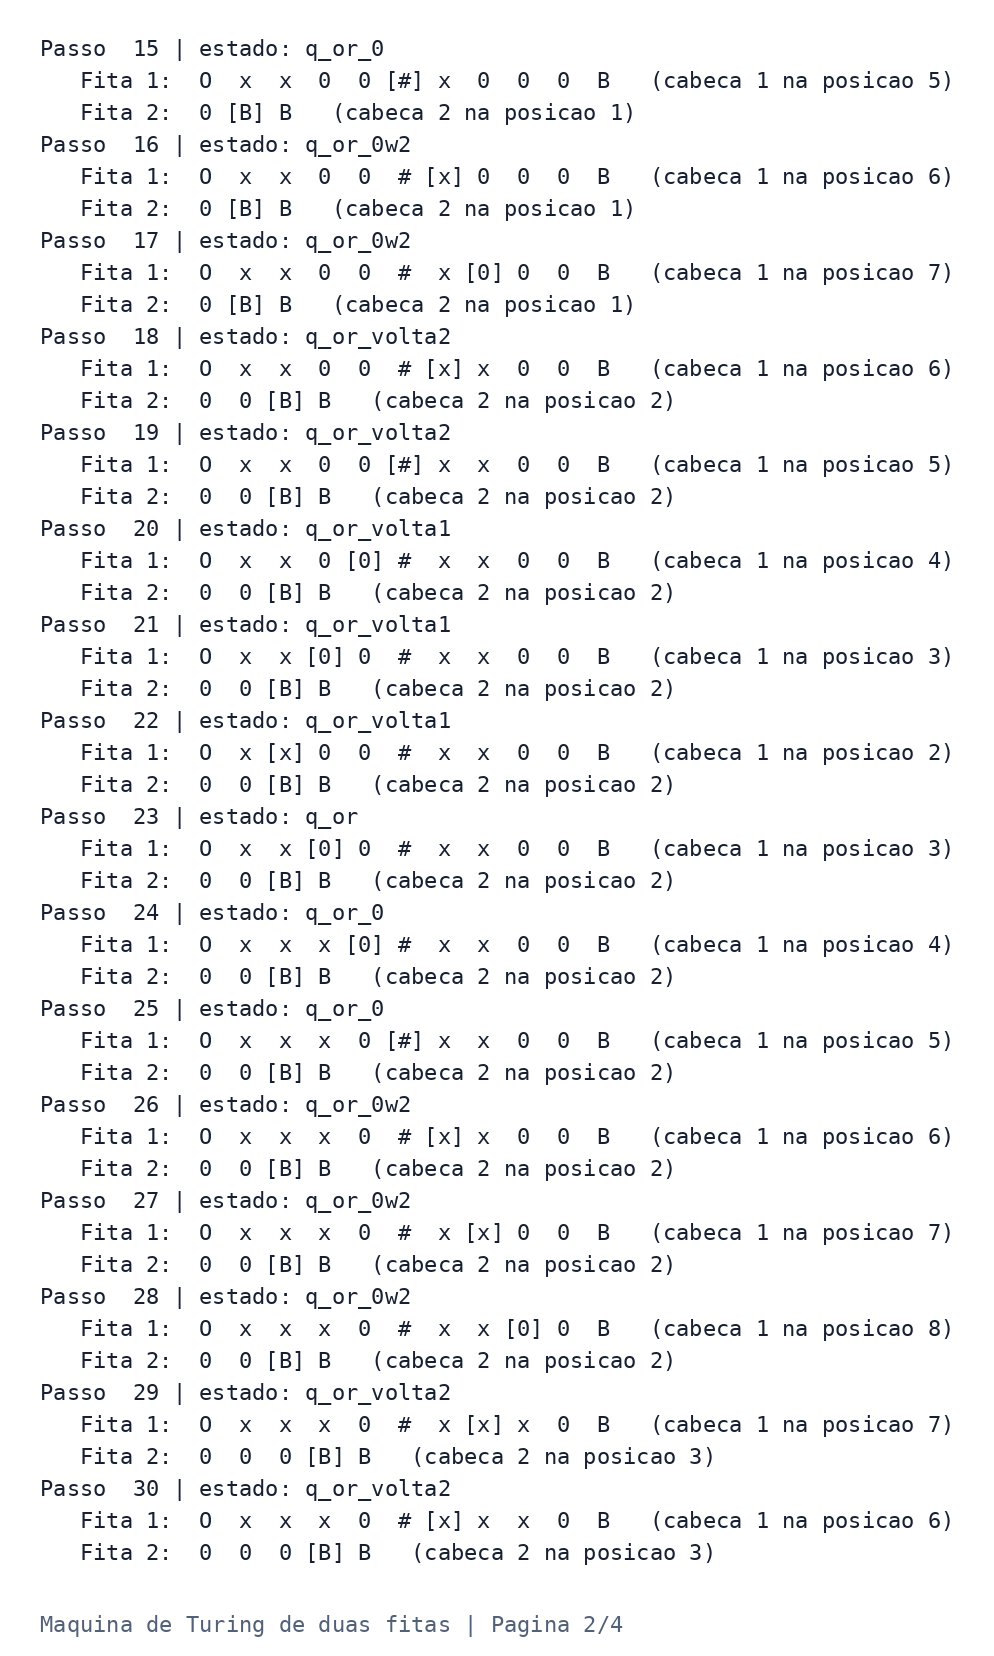
\includegraphics[width=\linewidth,height=0.78\textheight,keepaspectratio]{figuras/execucao/teste6_02.png}
\caption{Execução passo a passo da entrada \texttt{O0000\#0000} (esperado: \texttt{0000}) --- parte 2 de 4}
\end{figure}

\begin{figure}[H]
\centering
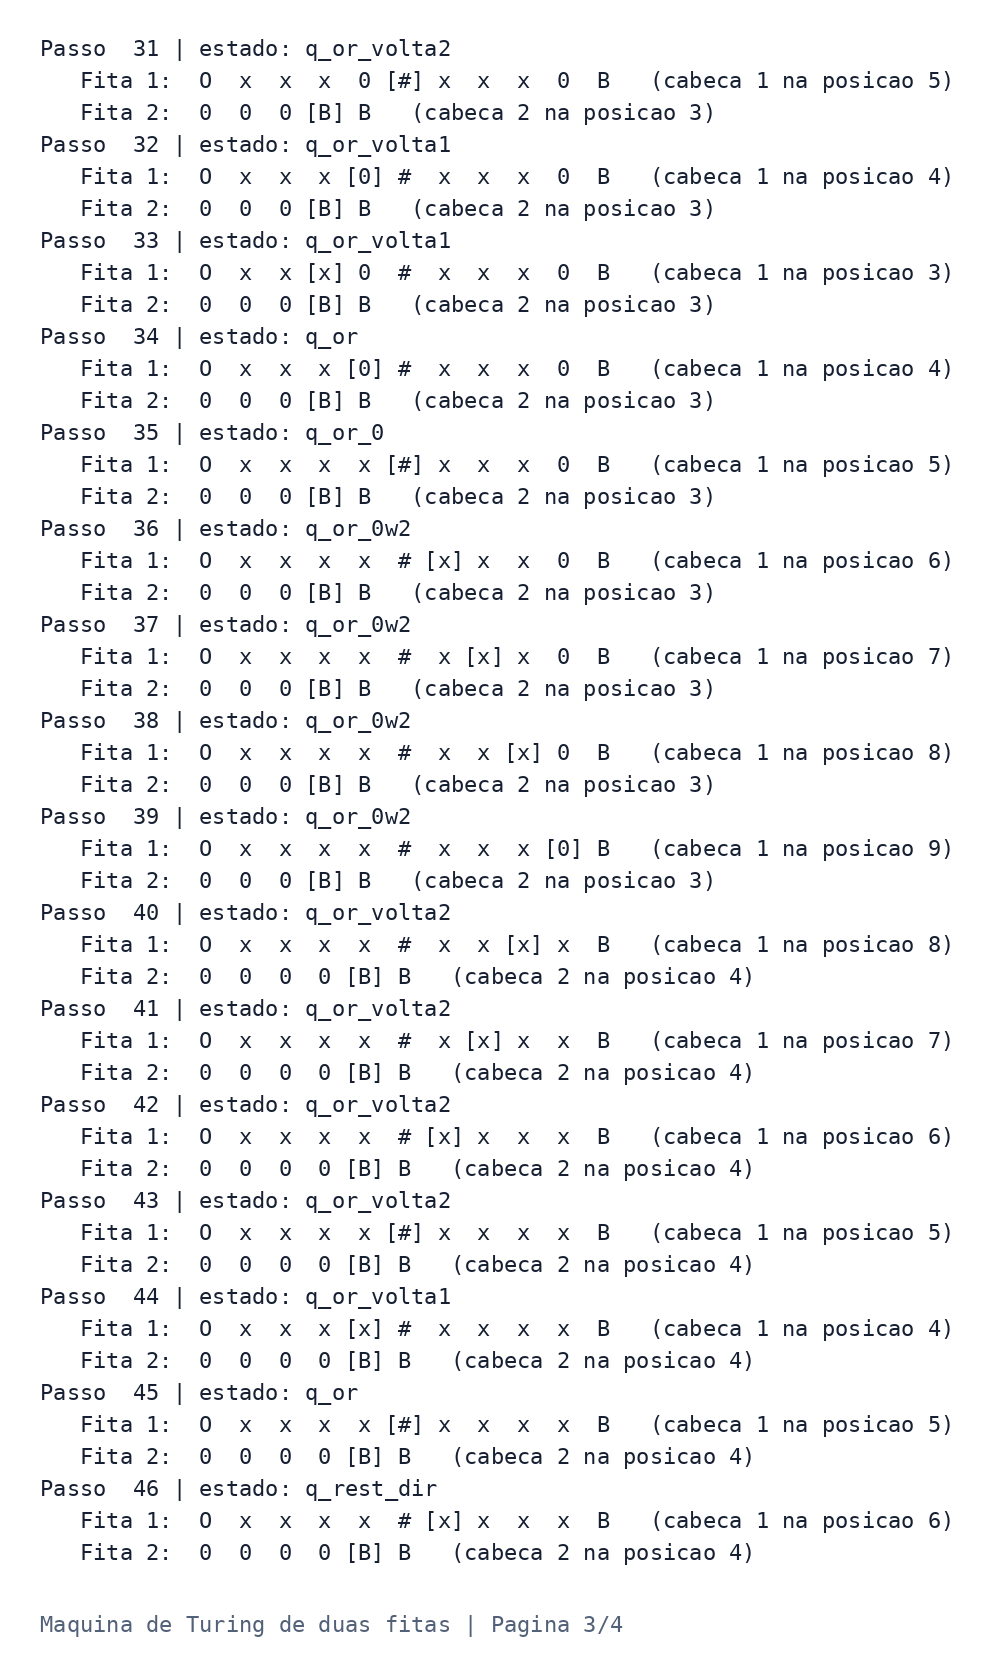
\includegraphics[width=\linewidth,height=0.78\textheight,keepaspectratio]{figuras/execucao/teste6_03.png}
\caption{Execução passo a passo da entrada \texttt{O0000\#0000} (esperado: \texttt{0000}) --- parte 3 de 4}
\end{figure}

\begin{figure}[H]
\centering
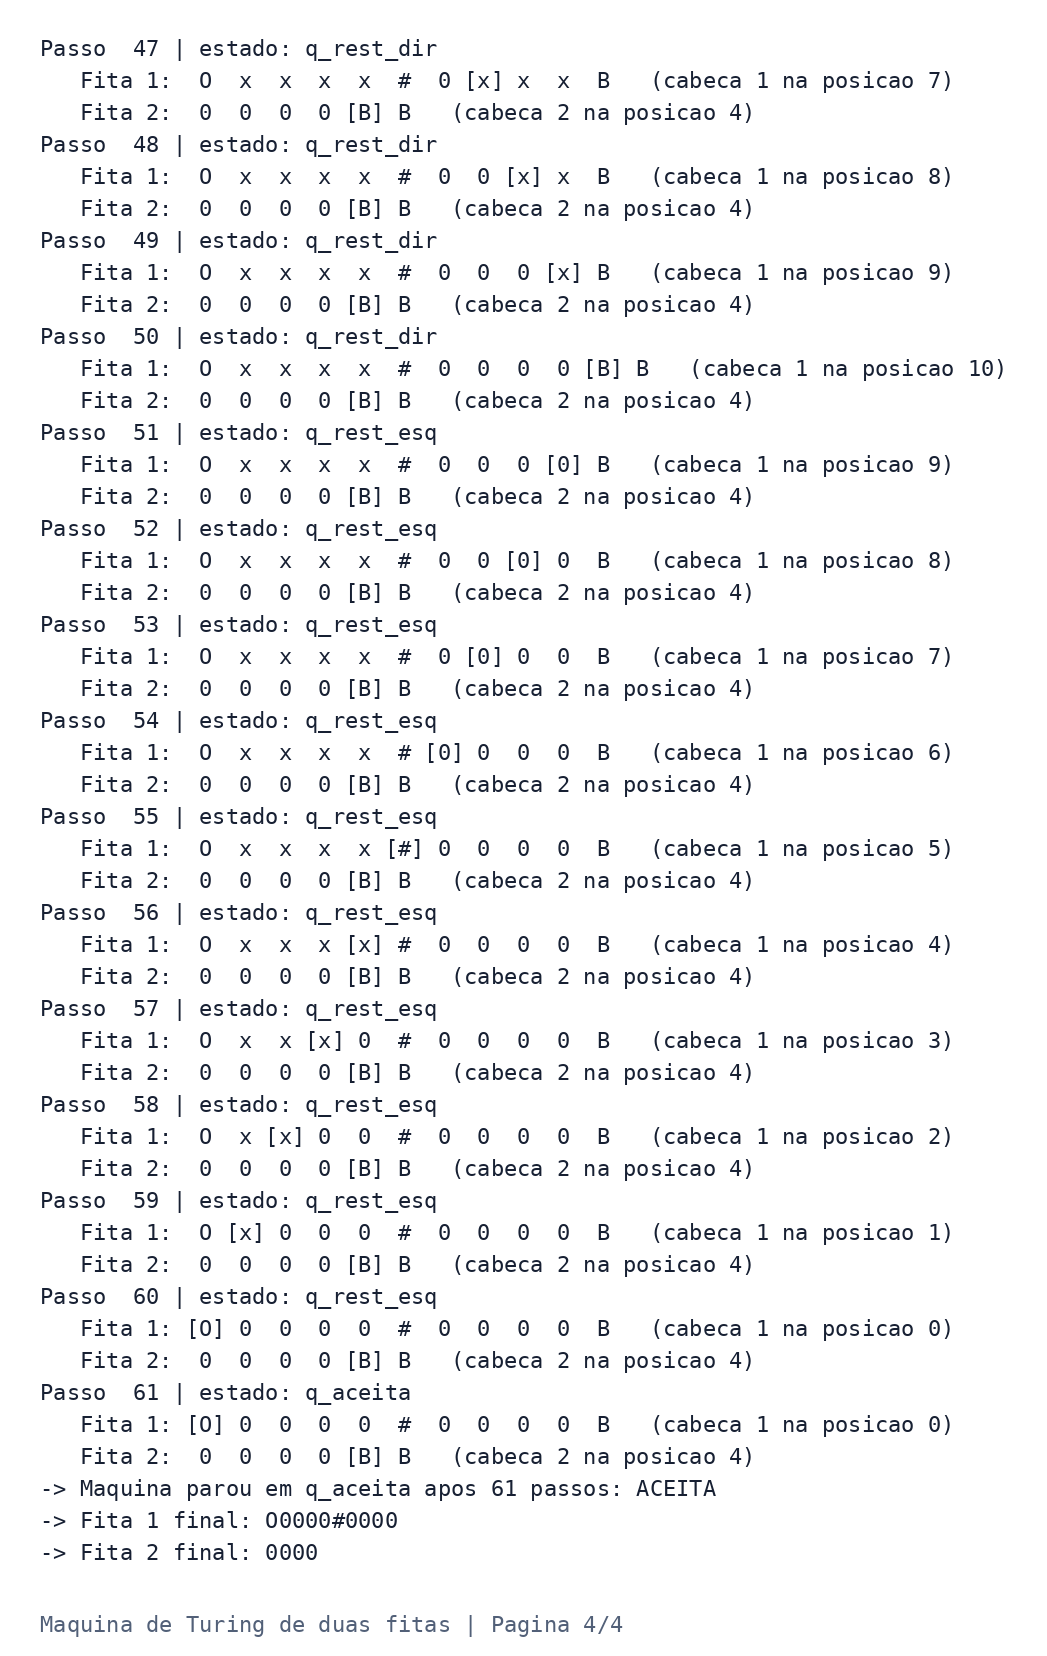
\includegraphics[width=\linewidth,height=0.78\textheight,keepaspectratio]{figuras/execucao/teste6_04.png}
\caption{Execução passo a passo da entrada \texttt{O0000\#0000} (esperado: \texttt{0000}) --- parte 4 de 4}
\end{figure}

% ── Teste 7: X01#11 → 10 ──────────────────────────────────────────
\subsection{Teste 7: \texttt{X01\#11}}
\label{sec:teste7}

\begin{figure}[H]
\centering
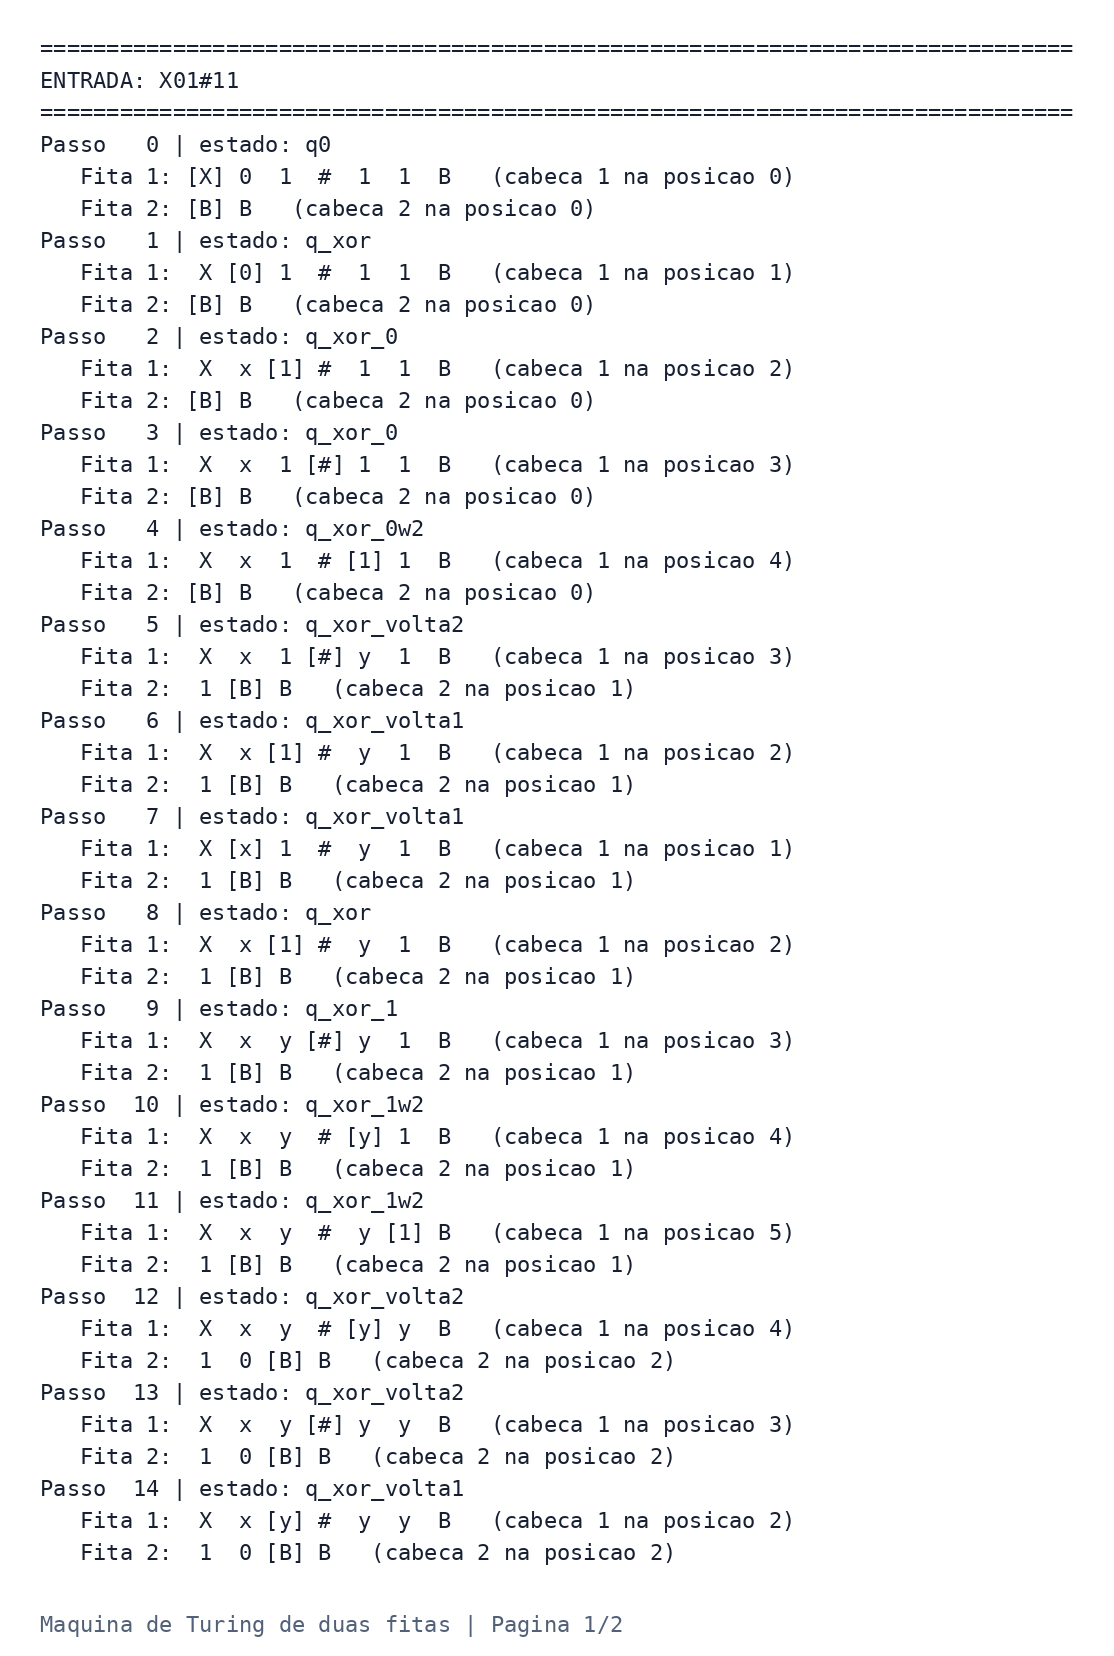
\includegraphics[width=\linewidth,height=0.78\textheight,keepaspectratio]{figuras/execucao/teste7_01.png}
\caption{Execução passo a passo da entrada \texttt{X01\#11} (esperado: \texttt{10}) --- parte 1 de 2}
\end{figure}

\begin{figure}[H]
\centering
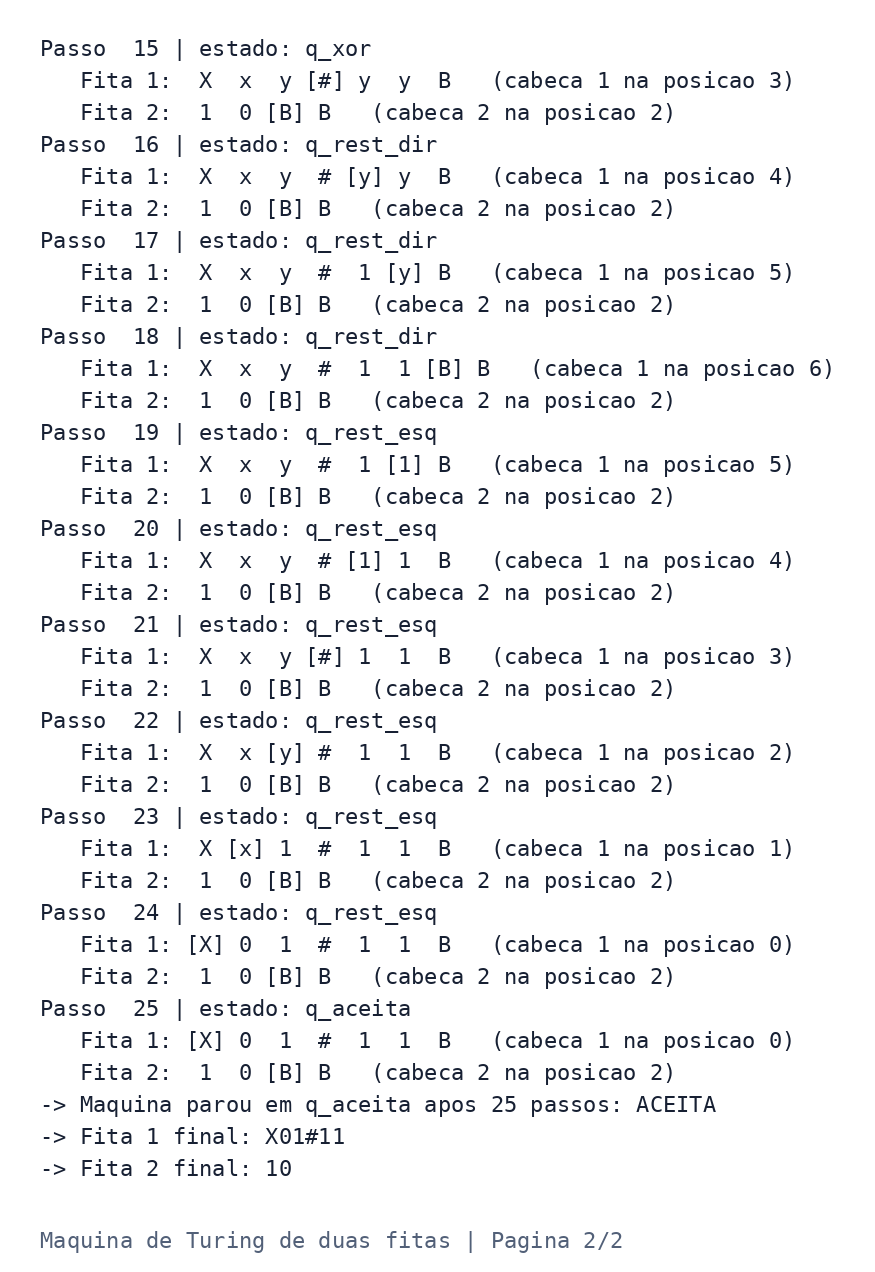
\includegraphics[width=\linewidth,height=0.78\textheight,keepaspectratio]{figuras/execucao/teste7_02.png}
\caption{Execução passo a passo da entrada \texttt{X01\#11} (esperado: \texttt{10}) --- parte 2 de 2}
\end{figure}

% ── Teste 8: X101#110 → 011 ───────────────────────────────────────
\subsection{Teste 8: \texttt{X101\#110}}
\label{sec:teste8}

\begin{figure}[H]
\centering
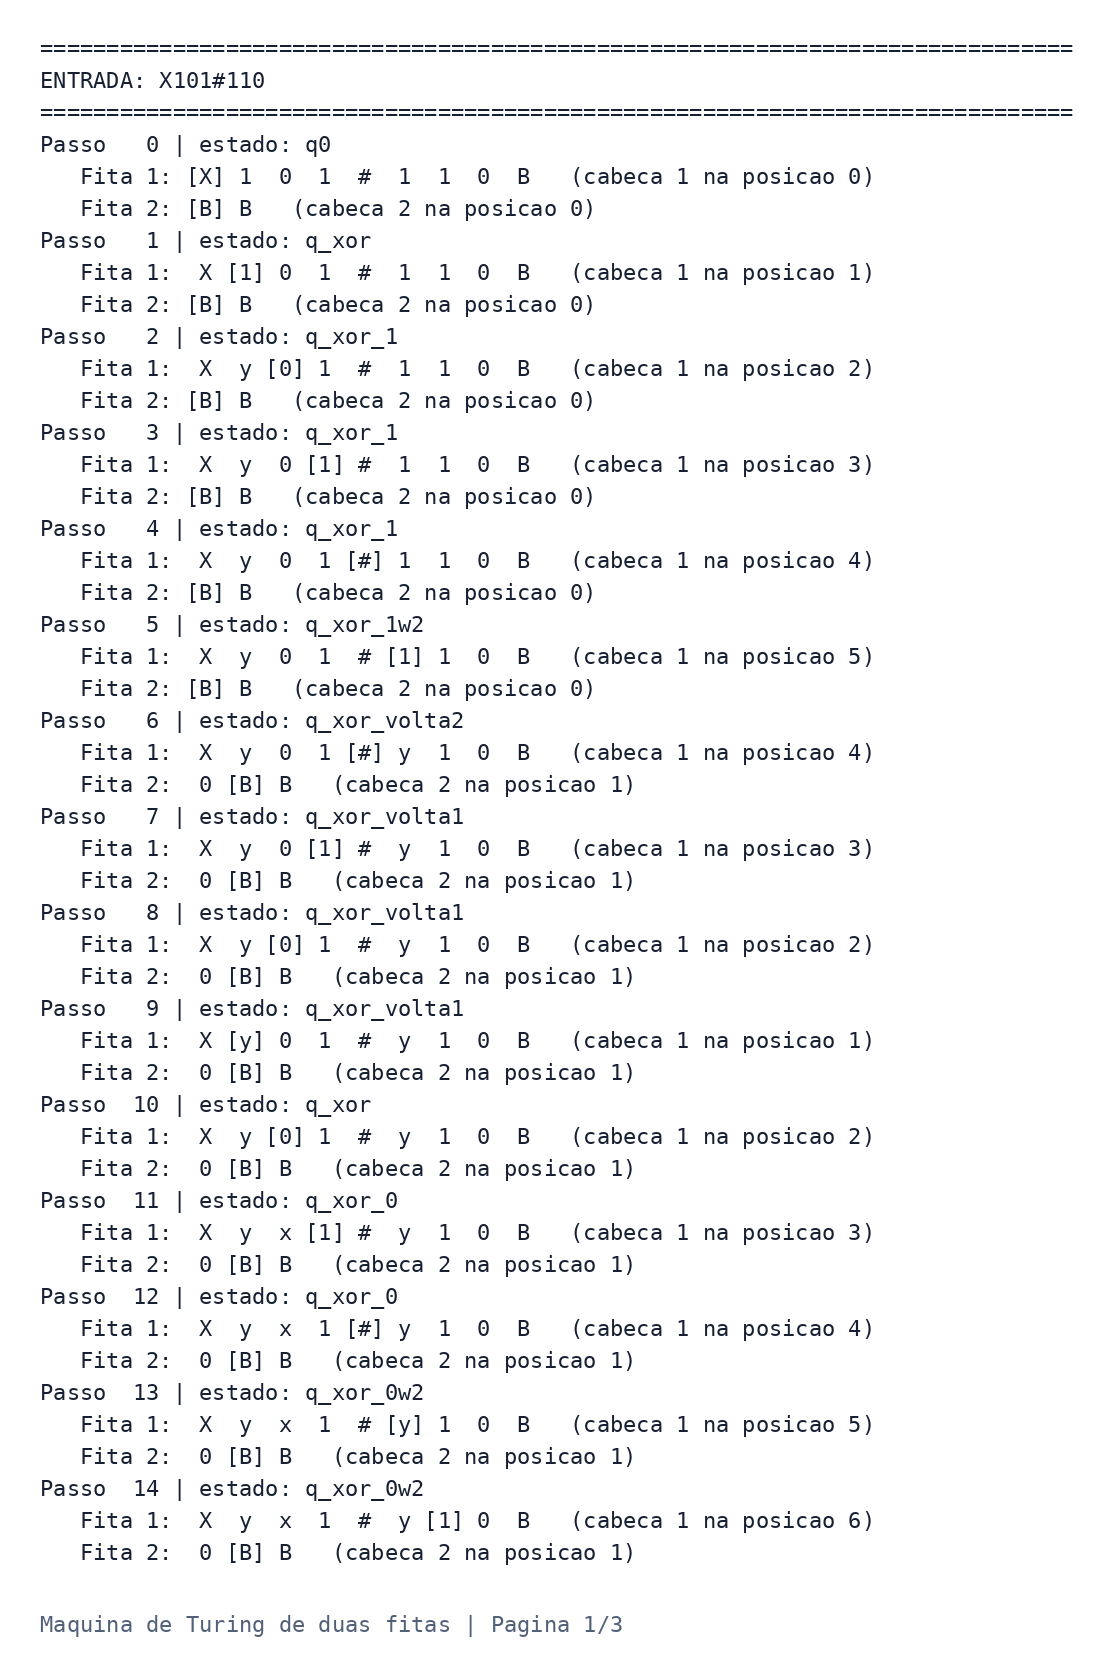
\includegraphics[width=\linewidth,height=0.78\textheight,keepaspectratio]{figuras/execucao/teste8_01.png}
\caption{Execução passo a passo da entrada \texttt{X101\#110} (esperado: \texttt{011}) --- parte 1 de 3}
\end{figure}

\begin{figure}[H]
\centering
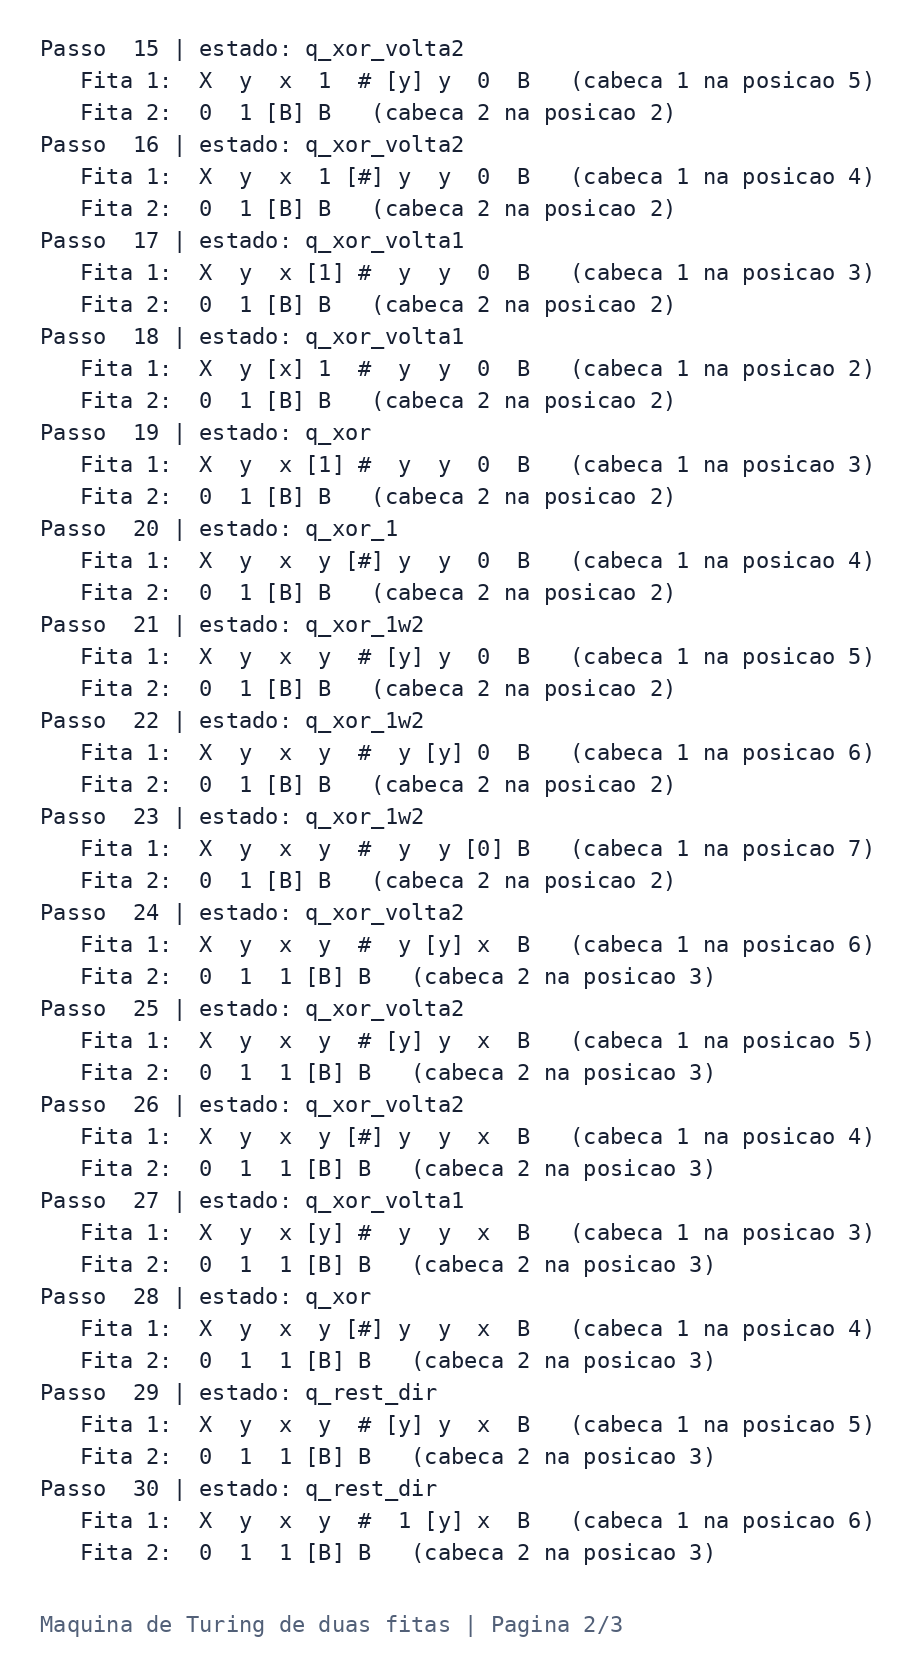
\includegraphics[width=\linewidth,height=0.78\textheight,keepaspectratio]{figuras/execucao/teste8_02.png}
\caption{Execução passo a passo da entrada \texttt{X101\#110} (esperado: \texttt{011}) --- parte 2 de 3}
\end{figure}

\begin{figure}[H]
\centering
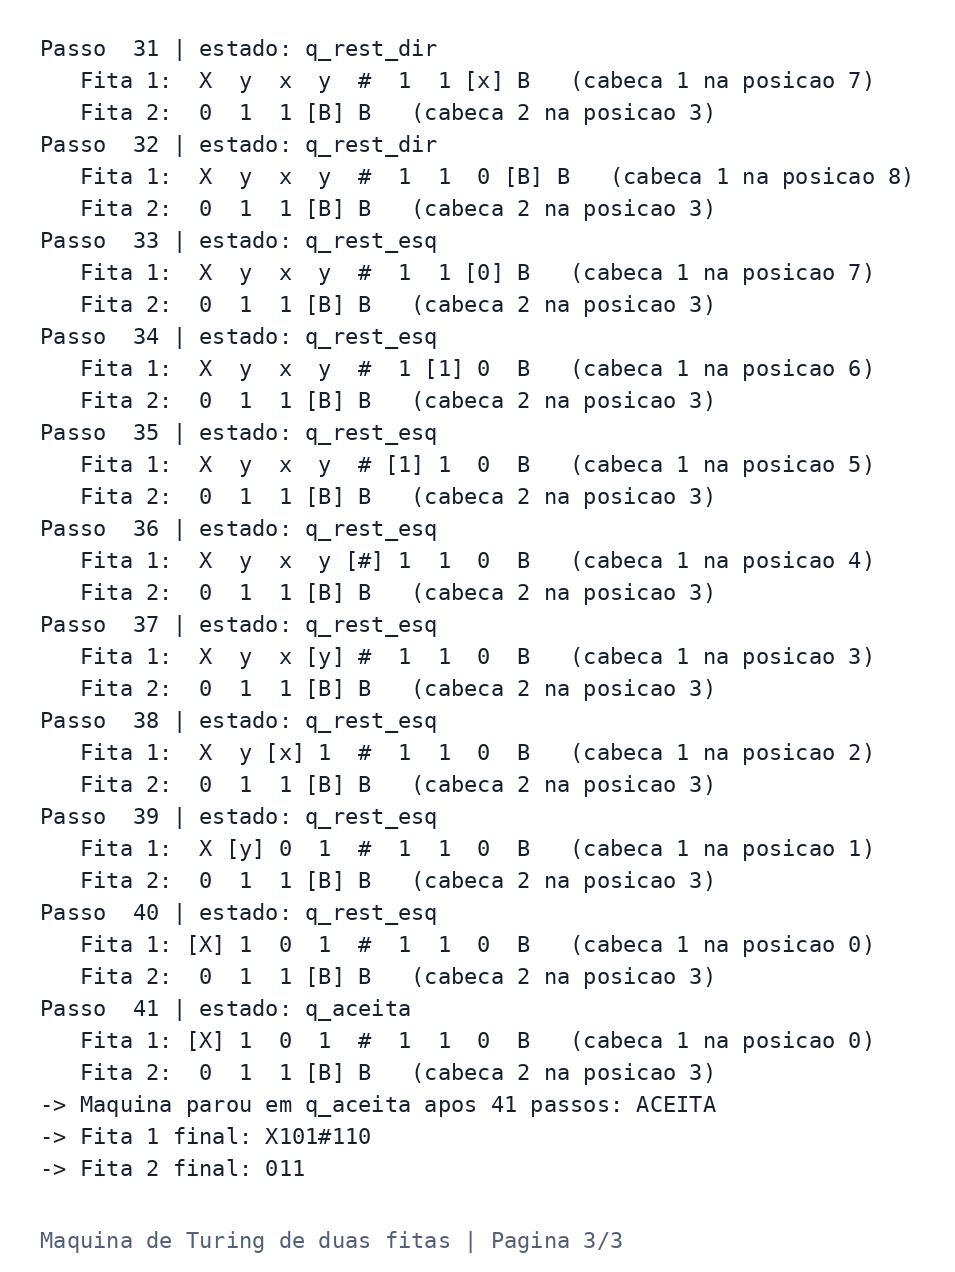
\includegraphics[width=\linewidth,height=0.78\textheight,keepaspectratio]{figuras/execucao/teste8_03.png}
\caption{Execução passo a passo da entrada \texttt{X101\#110} (esperado: \texttt{011}) --- parte 3 de 3}
\end{figure}

% ── Teste 9: X1100#1010 → 0110 ────────────────────────────────────
\subsection{Teste 9: \texttt{X1100\#1010}}
\label{sec:teste9}

\begin{figure}[H]
\centering
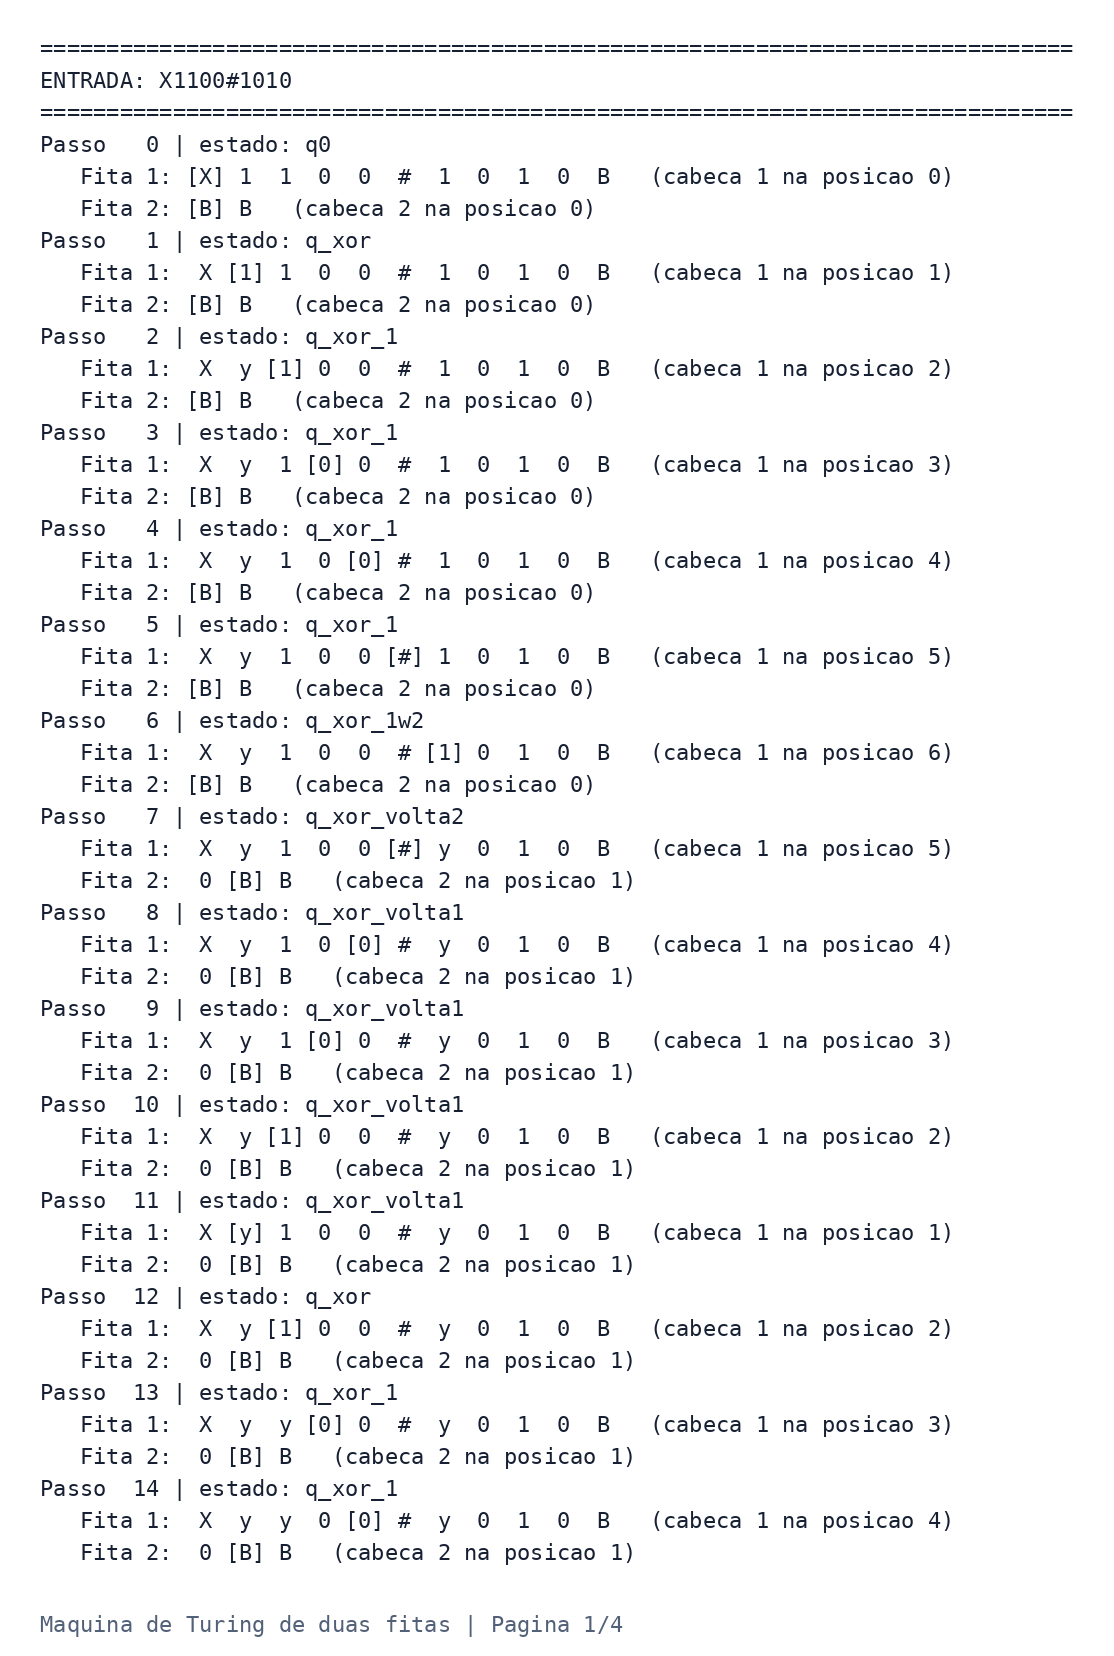
\includegraphics[width=\linewidth,height=0.78\textheight,keepaspectratio]{figuras/execucao/teste9_01.png}
\caption{Execução passo a passo da entrada \texttt{X1100\#1010} (esperado: \texttt{0110}) --- parte 1 de 4}
\end{figure}

\begin{figure}[H]
\centering
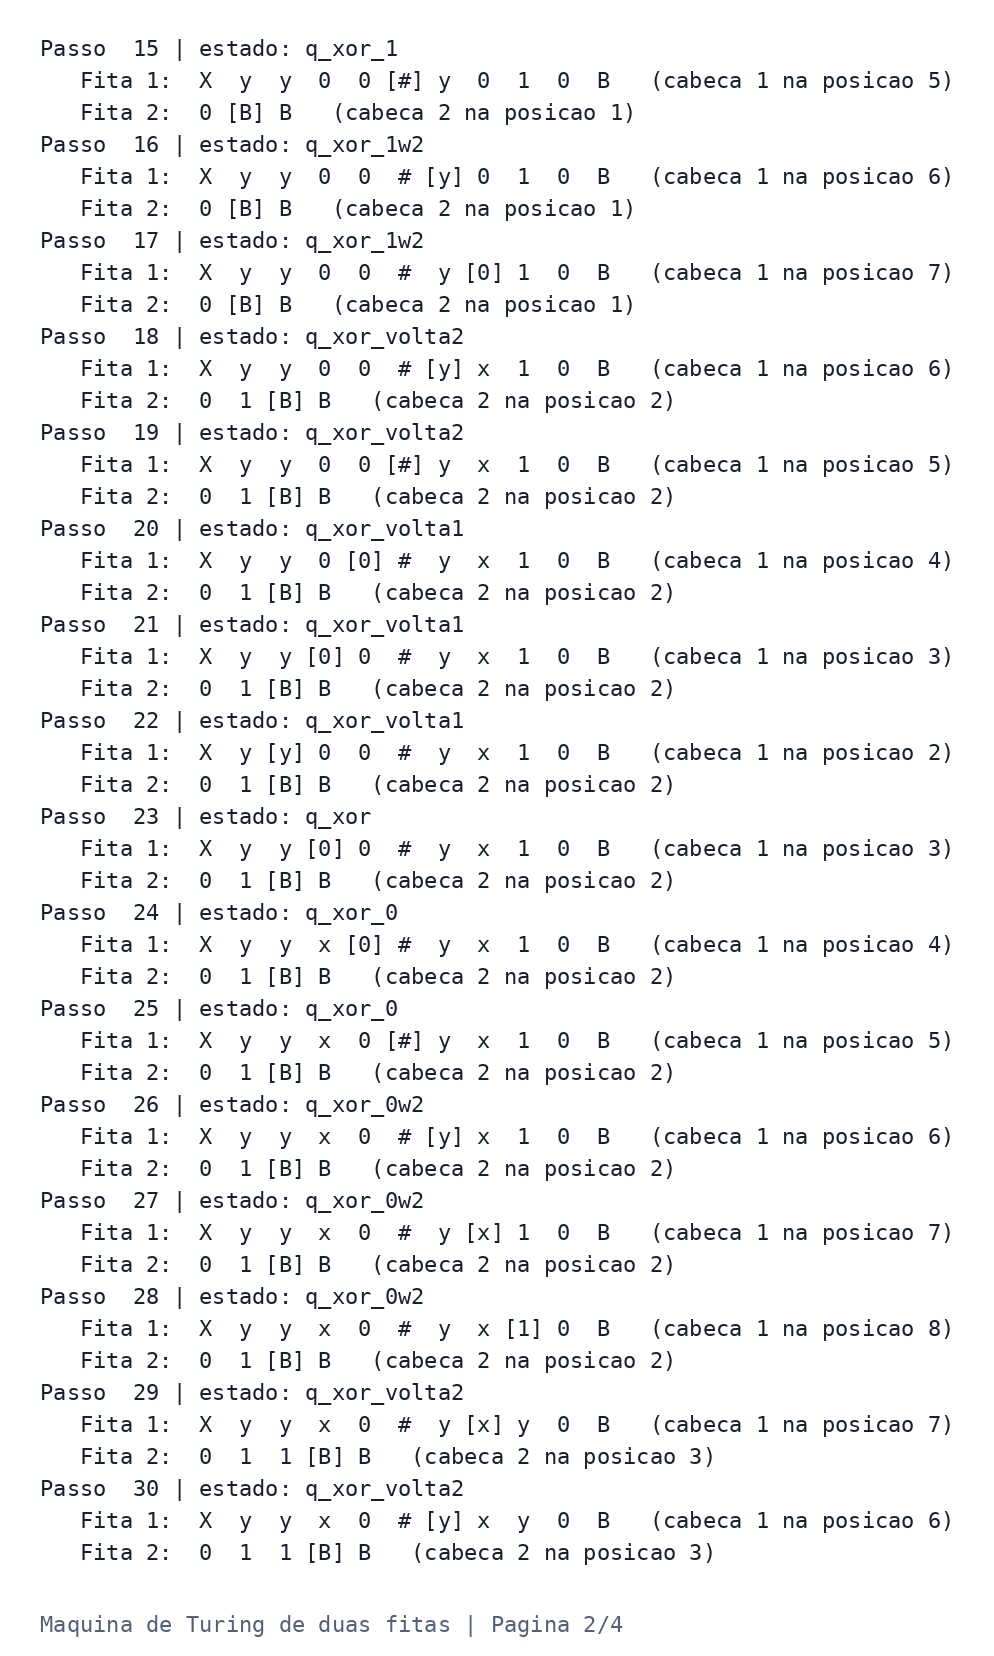
\includegraphics[width=\linewidth,height=0.78\textheight,keepaspectratio]{figuras/execucao/teste9_02.png}
\caption{Execução passo a passo da entrada \texttt{X1100\#1010} (esperado: \texttt{0110}) --- parte 2 de 4}
\end{figure}

\begin{figure}[H]
\centering
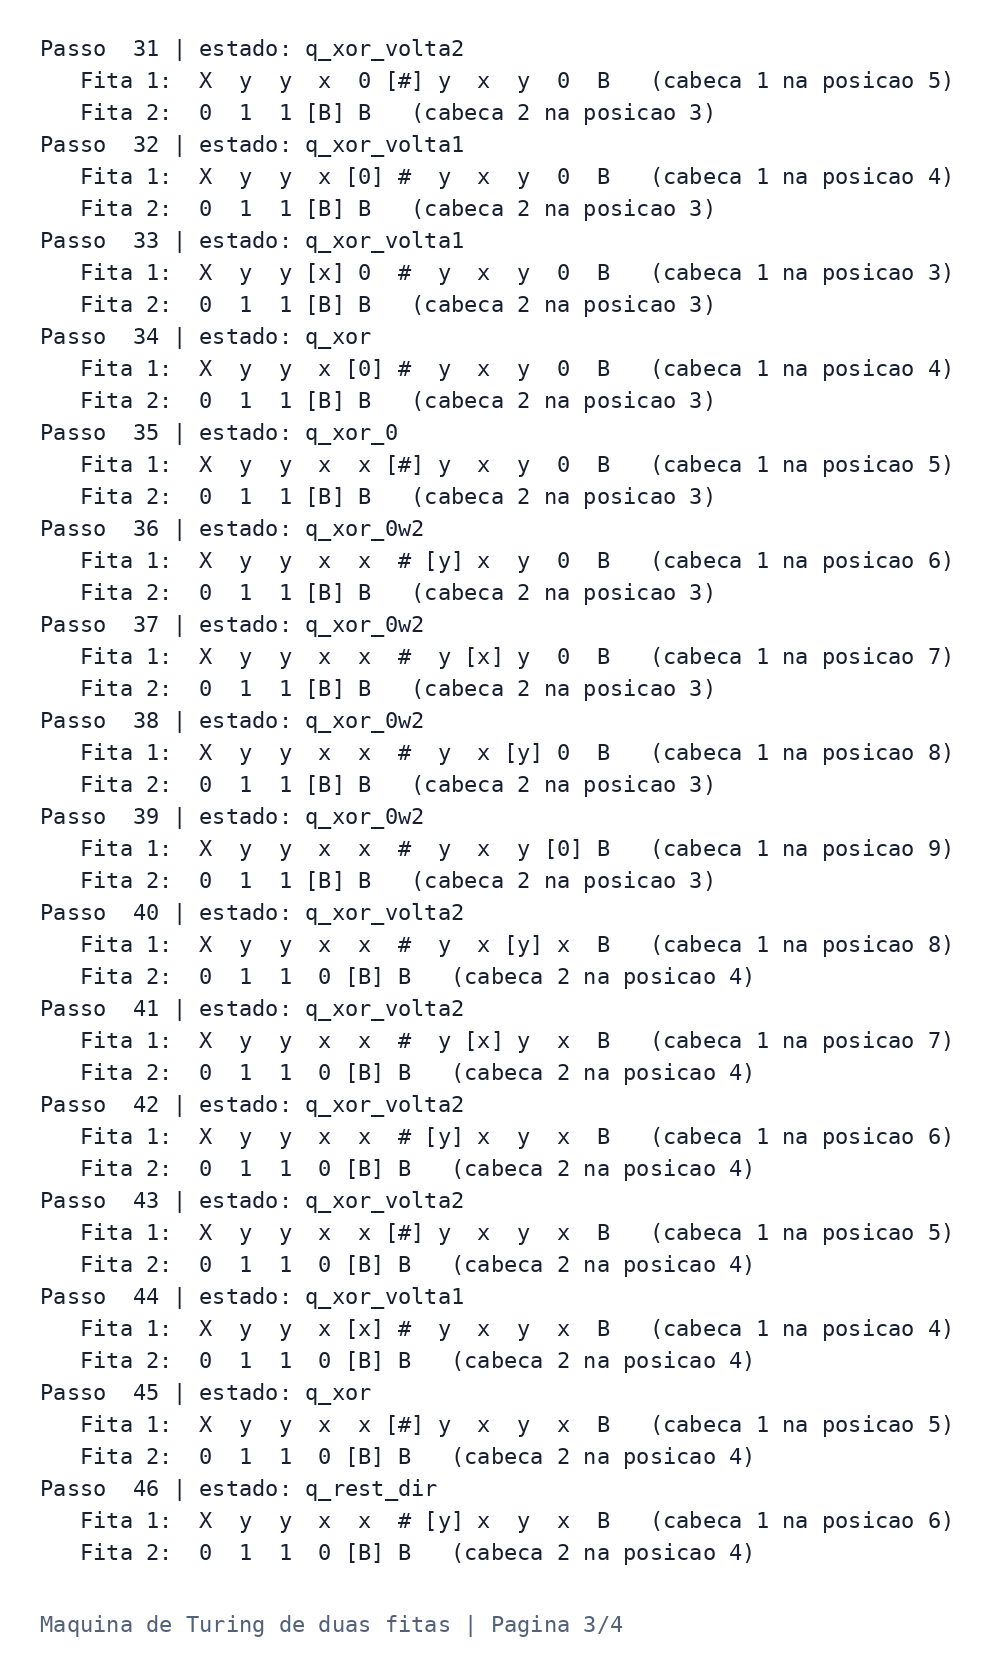
\includegraphics[width=\linewidth,height=0.78\textheight,keepaspectratio]{figuras/execucao/teste9_03.png}
\caption{Execução passo a passo da entrada \texttt{X1100\#1010} (esperado: \texttt{0110}) --- parte 3 de 4}
\end{figure}

\begin{figure}[H]
\centering
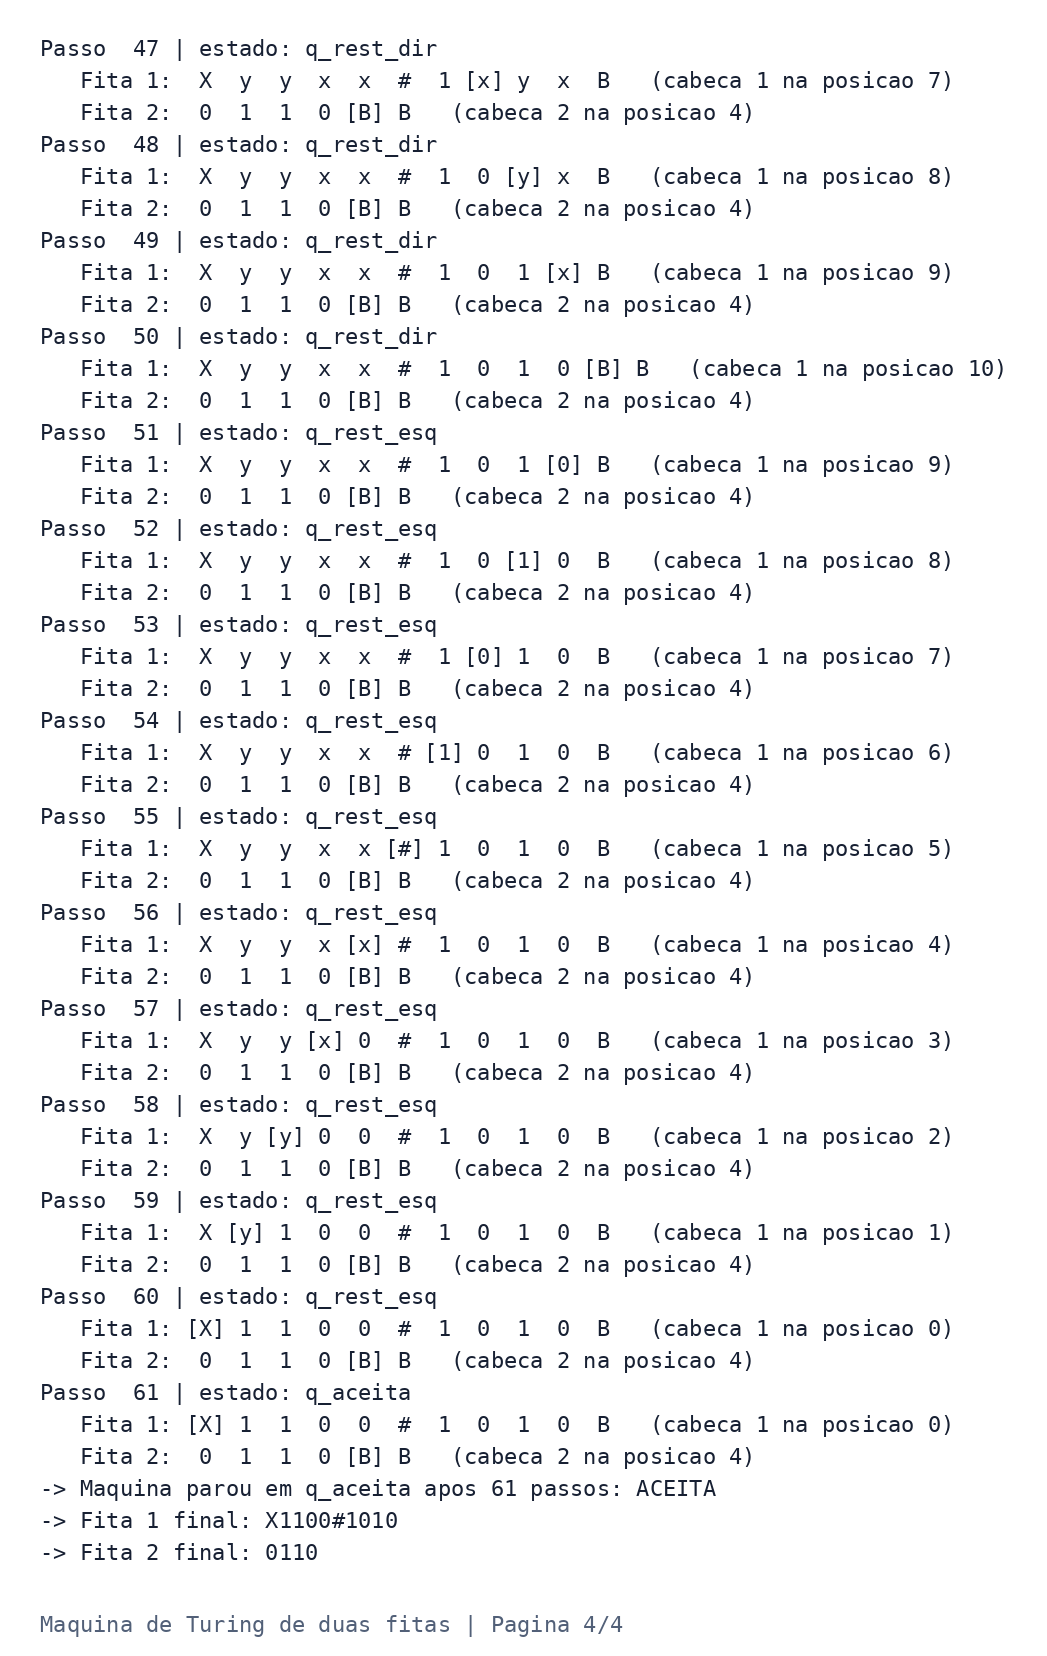
\includegraphics[width=\linewidth,height=0.78\textheight,keepaspectratio]{figuras/execucao/teste9_04.png}
\caption{Execução passo a passo da entrada \texttt{X1100\#1010} (esperado: \texttt{0110}) --- parte 4 de 4}
\end{figure}
\clearpage

\bibliographystyle{plain}
\bibliography{referencias}

\end{document}
